

Questo dataset consiste di una simulazione di MD eseguita con QE per una struttura cristallina costituita da \ce{Ta2O5}, pentossido di ditantalio (a cui ci riferiamo anche come tantala). 


Esso è composto da una serie di file di QE che costituiscono la dinamica molecolare di una struttura di tantala a circa 3000K.

Usando la libreria ASE abbiamo generato una rappresentazione della cella atomica dai dati di QE analizzati, essendo una simulazione di dinamica molecolare, riportiamo solo uno degli step, a cui diamo il nome di frame. Riportiamo di seguito questa immagine, disegnata tramite matplotlib \ref{fig:cristallo-from-ase-frame-0-dataset-a}.

\begin{figure}[h]
    \centering
    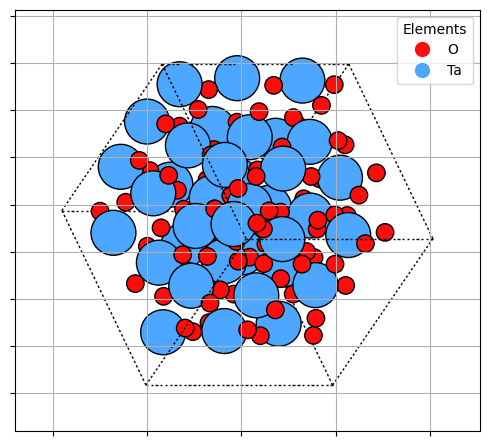
\includegraphics[scale=0.5]{./img/cristallo-from-ase-frame-0-dataset-a.png}
    \caption{Rappresentazione generata tramite ASE della struttura atomica del dataset A}
    \label{fig:cristallo-from-ase-frame-0-dataset-a}
\end{figure}


\section{SOAP con DScribe}

Considerando la discussione svolta per spiegare SOAP unita alla spiegazione riguardante DScribe, vogliamo dare un esempio pratico di utilizzo del metodo considerando un contesto sul quale conosciamo già il risultato.

Dove abbiamo utilizzato \autoref{code:soap-dscribe} nel seguente modo

\begin{lstlisting}[caption={Snippet usato per il detaset A}, label={code:soap-dataset-a}, language=Python]
    soap_obj = SOAP(
        species=["Ta", "O"],
        periodic=True,       
        r_cut=5.0,      
        n_max=8,         
        l_max=6 
    )
    
    features = soap_obj.create(QE_data, n_jobs=-1)
\end{lstlisting}

\subsubsection{Nota sui parametri}
Dato che ci stiamo ponendo come scopo quello di verificare che il metodo sia utilizzabile, i parametri riportati sopra non sono stati in alcun modo ottimizzati, essi sono stati reperiti negli esempi della documentazione grazie a strumenti di AI che ne hanno fatto la revisione. 
Data la spiegazione che abbiamo dato per essi, il test che si potrebbe svolgere per la loro ottimizzazione è un tradeoff tra velocità di calcolo e accurateza dei risultati rispetto a quelli prodotti da Quantum Espresso.
\\



Consideriamo l'atomo 42 e calcoliamo un \textit{kernel} tra i frame successivi, questo significa che seguiamo un singolo atomo lungo tutta la dinamica molecolare.

Un kernel è una funzione che ci permette di misurare quanto due descrittori soap (il power spectrum) siano simili, e conseguentemente gli ambienti da cui derivano. Nel nostro caso usiamo il kernel più semplice possibile:

\begin{equation}
    \mathrm{Kernel}(\vec{p_1},\vec{p_2}) = \frac{\vec{p_1}\cdot\vec{p_2}}{|\vec{p_1}|\,|\vec{p_2}|}
    \label{eq:kernel-lineare}
\end{equation}

Il risultato che ci aspettiamo è che lungo tutti i frame il valore di questa funzione sia circa uno, data la struttura dei dati, infatti ogni frame rappresenta un piccolo scostamento temporale di una dinemica molecolare continua.

Se produciamo un grafico dove lungo l'asse x poniamo un indice (1 rappresenta il confrnto tra il frame 1 e 2, e così per tutti gli altri indici) e sull'asse delle y mettiamo il valore del kernel ottenimo:

\begin{figure}[h]
    \centering
    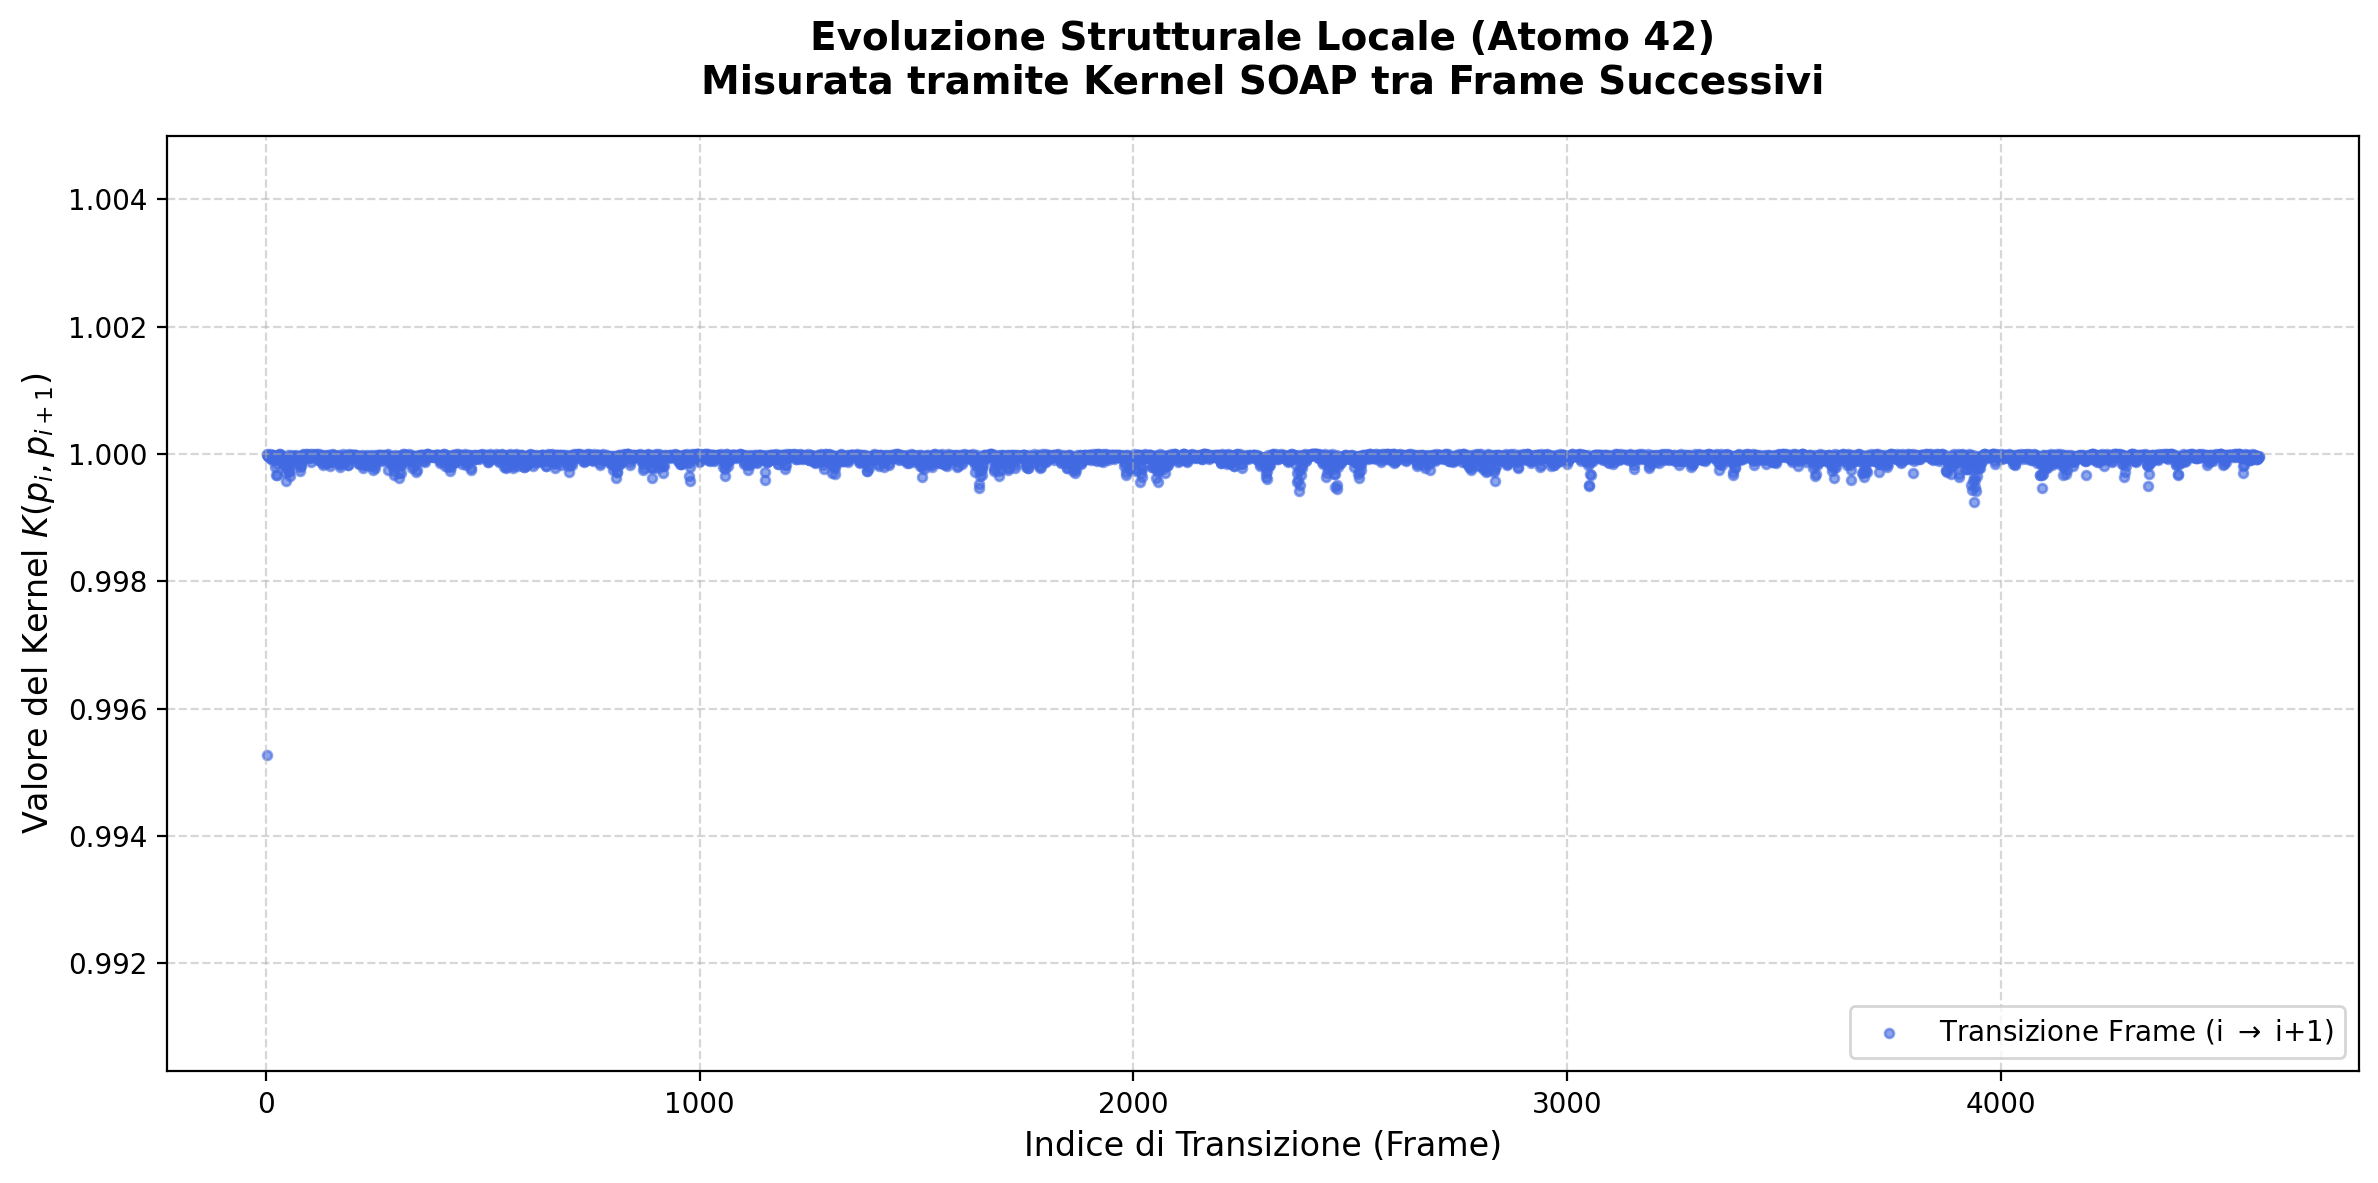
\includegraphics[scale=0.5]{./img/kernel.png}
    \caption{Rappresentazione del kernel per i frame del Datase A}
    \label{fig:kernel-dataset-a}
\end{figure}

Il risultato è esattamente quello atteso, l'unico punto che si discosta è il primo, non riteniamo questo punto particolarmente problematico.
\\

\section{Prima sessione di testing}
In questa sezione spiegheremo come è stato utilizzato il dataset A per sperimentare il funzionamento del workflow descritto all'inizio del documento.

\subsection{Addestramento potenziale con Quippy}

\begin{lstlisting}[caption={Snippet usato per il calcolo del GAP per il detaset A}, label={code:gap-dataset-a}, language=bash]

    gap_fit 
    at_file=train_data.extxyz 
    default_sigma={0.0002 0.1 0.0 0.0} 
    gap={soap 
        l_max=2 
        n_max=2 
        atom_sigma=0.5 
        zeta=4 
        cutoff=5.0 
        covariance_type=dot_product 
        n_sparse=500 
        sparse_method=cur_points
        delta=1
        } 
    e0={Ta:-9884.889316093:O:-561.82449957} 
    energy_parameter_name=energy 
    force_parameter_name=forces 
    gp_file=out_potenziale_gap-500-n2-l2.xml
    > potenziale_quippy-500-n2-l2.log

\end{lstlisting}



\subsubsection{Nota sui parametri}
Dato che ci stiamo ponendo come scopo quello di verificare che il metodo sia utilizzabile, i parametri riportati sopra non sono stati in alcun modo ottimizzati, essi sono stati reperiti negli esempi della documentazione grazie a strumenti di AI che ne hanno fatto la revisione. 
Data la spiegazione che abbiamo dato per essi, il test che si potrebbe svolgere per la loro ottimizzazione è un tradeoff tra velocità di calcolo e accurateza dei risultati rispetto a quelli prodotti da Quantum Espresso.

Per l'errore relativo alle energie, abbiamo usato lo stesso ordine di grandezza che quantum espresso utilizzava per decretare la convergenza della simulazione.
Le energie per gli atomi isolati \texttt{e0} sono state determinate tramite una simulazione di QE.
Il grado in \texttt{n} e \texttt{l} per le armoniche sferiche sono stati impostati come tali per la limitatezza della RAM disponibile sul sistema usato per il training, i problemi relativi all'accuratezza dei dati, come si può vedere sotto, in prima analisi possono essere imputabili a queta brusca approssimazione.


La nomenclatura dei parametri è standard e deriva dall'aver prodotto il file con ASE.

Gli altri parametri, come detto sono stati forniti dalla documentazione e andrebbero ottimizzati. Non escludiamo che possano esserci problemi di accuratezza dovuti alla scelta i questi valori.


\subsection{Verifica delle energie}

Per verificare se il potenziale così addestrato sia in grado di predirre in modo corretto le energie abbiamo estratto le configurazioni geometriche prodotte da Quantum Espresso e utilizzato il potenziale addestrato per predirre l'energia, successivamente abbiamo confrontato i valori predetti con quelli calcolati da Quantum Espresso.

\subsubsection{Training set}

Per prima cosa verifichiamo se utilizzando come dati di input quelli usati durante la fase di addestramento otteniamo il risultato atteso, se così non fosse potremmo velocemente concludere che l'addestramento non è andato a buon fine.

\begin{figure}[h]
    \centering
    
\includegraphics[scale=0.5]{./img/parity_plot_gap_vs_qe-traindata.png}
    \caption{Confronto tra i valori di energia potenziale predetti dal potenziale GAP e quelli calcolati tramite Quantum Espresso}
    \label{fig:parity_plot_gap_vs_qe-traindata}
\end{figure}

Dal grafico sopra possiamo vedere che il risultato è compatibile con le aspettative, e le energie predettre assomigliano a quelle prodotte da Qauntum Espresso.


\subsubsection{Test set}

In questa fase invece vogliamo verificare come si comporta il potenziale nel caso di dati su cui non è stato addestrato, ricordiamo che questo set è composto dalla seconda metà della dinamica totale descritta dalla totalità del dataset A.

\begin{figure}[h]
    \centering
    
\includegraphics[scale=0.5]{./img/parity_plot_gap_vs_qe-testdata.png}
    \caption{Confronto tra i valori di energia potenziale predetti dal potenziale GAP e quelli calcolati tramite Quantum Espresso}
    \label{fig:parity_plot_gap_vs_qe-testdata}
\end{figure}

Possiamo vedere che i risultati non si allineano perfettamente con le aspettative, ma date le limitazioni dei parametri di addestramento del potenziale e dalla rapidità di calcolo ottenuta, possiamo considerare questo un buon risultato iniziale.


\subsection{Verifica delle forze}

Oltre a verificare le energie abbiamo deciso di verificare anche le forze. Abbiamo estratto le forze da Quantum Espresso da utilizzare come reference, successivamente abbiamo determinato il valore delle forze usando il potenziale addestrato a partire dalle configurazioni usate da Quantum Espresso.

\subsubsection{Training set}

Il seguente grafico mostra il confronto tra le forze calcolate da Qauntum Espresso e quelle predette dal potenziale, essendo queste le configurazioni usate nel training ci aspettiamo un buon accordo.

\begin{figure}[h]
    \centering
    
\includegraphics[scale=0.4]{./img/parity_plot_forze-traindata.png}
    \caption{Confronto, suddiviso per asse di riferimento, tra i valori di forza calcolati a partire da Qauntum Espresso e dal potenziale addestrato}
    \label{fig:parity_plot_forze-traindata}
\end{figure}


\subsubsection{Test set}

Procediamo adesso come sopra ad utilizzare l'altra parte del dataset per verificare la compatibilità tra calcolo e predizioni.

\begin{figure}[h]
    \centering
    
\includegraphics[scale=0.4]{./img/parity_plot_forze-testdata.png}
    \caption{Confronto, suddiviso per asse di riferimento, tra i valori di forza calcolati a partire da Qauntum Espresso e dal potenziale addestrato}
    \label{fig:parity_plot_forze-testdata}
\end{figure}

anche in questo caso i risultati mostra un buon accordo.

Possiamo ipotizzare che questo grado di accordo superiore rispetto alle energie, sia almeno in parte dovuto al fatto che l'errore stima per le energie, e inserito nei parametri di affestramento del potenziale, è di tre ordini di grandezza superiore.



\section{Simulazione NVE}

Abbiamo provato ad effettuare una simulazione di tipo NVE, costruita al seguente modo. Dai file di QE per il set di test abbiamo estratto la configurazione spaziale iniziale degli atomi.
Questa struttura è stata utilizzata come punto di partenza per il calcolo di energie e forze, la sua evoluzione darà poi configurazioni diverse rispetto a quelle prodotte da QE.
Seguendo la struttura descritta precedentemente abbiamo impostato la simulazione con i seguenti parametri, timestep pari a $4.8$fs, come quello usato in Quantum Espresso, e un totale di $2'000$ step.
Come detto, data la diversa configurazione i risultati non possono essere confrontati direttamente con quelli prodotti da QE. 
Per verificare la stabilità dei risultati facciamo un grafico della temepratura e dell'energia in funzione dello step temporale.
Abbiamo provato a reperire i valori delle velocità iniziali dal file di output di QE, ma non essendo presenti, le abbiamo estratte da una distribuzione di Maxwell-Boltzman per una temperatura di $3'000$K.
\\

I risultati di energia e temperatura che otteniamo sono i seguenti

\begin{figure}[h]
    \centering
    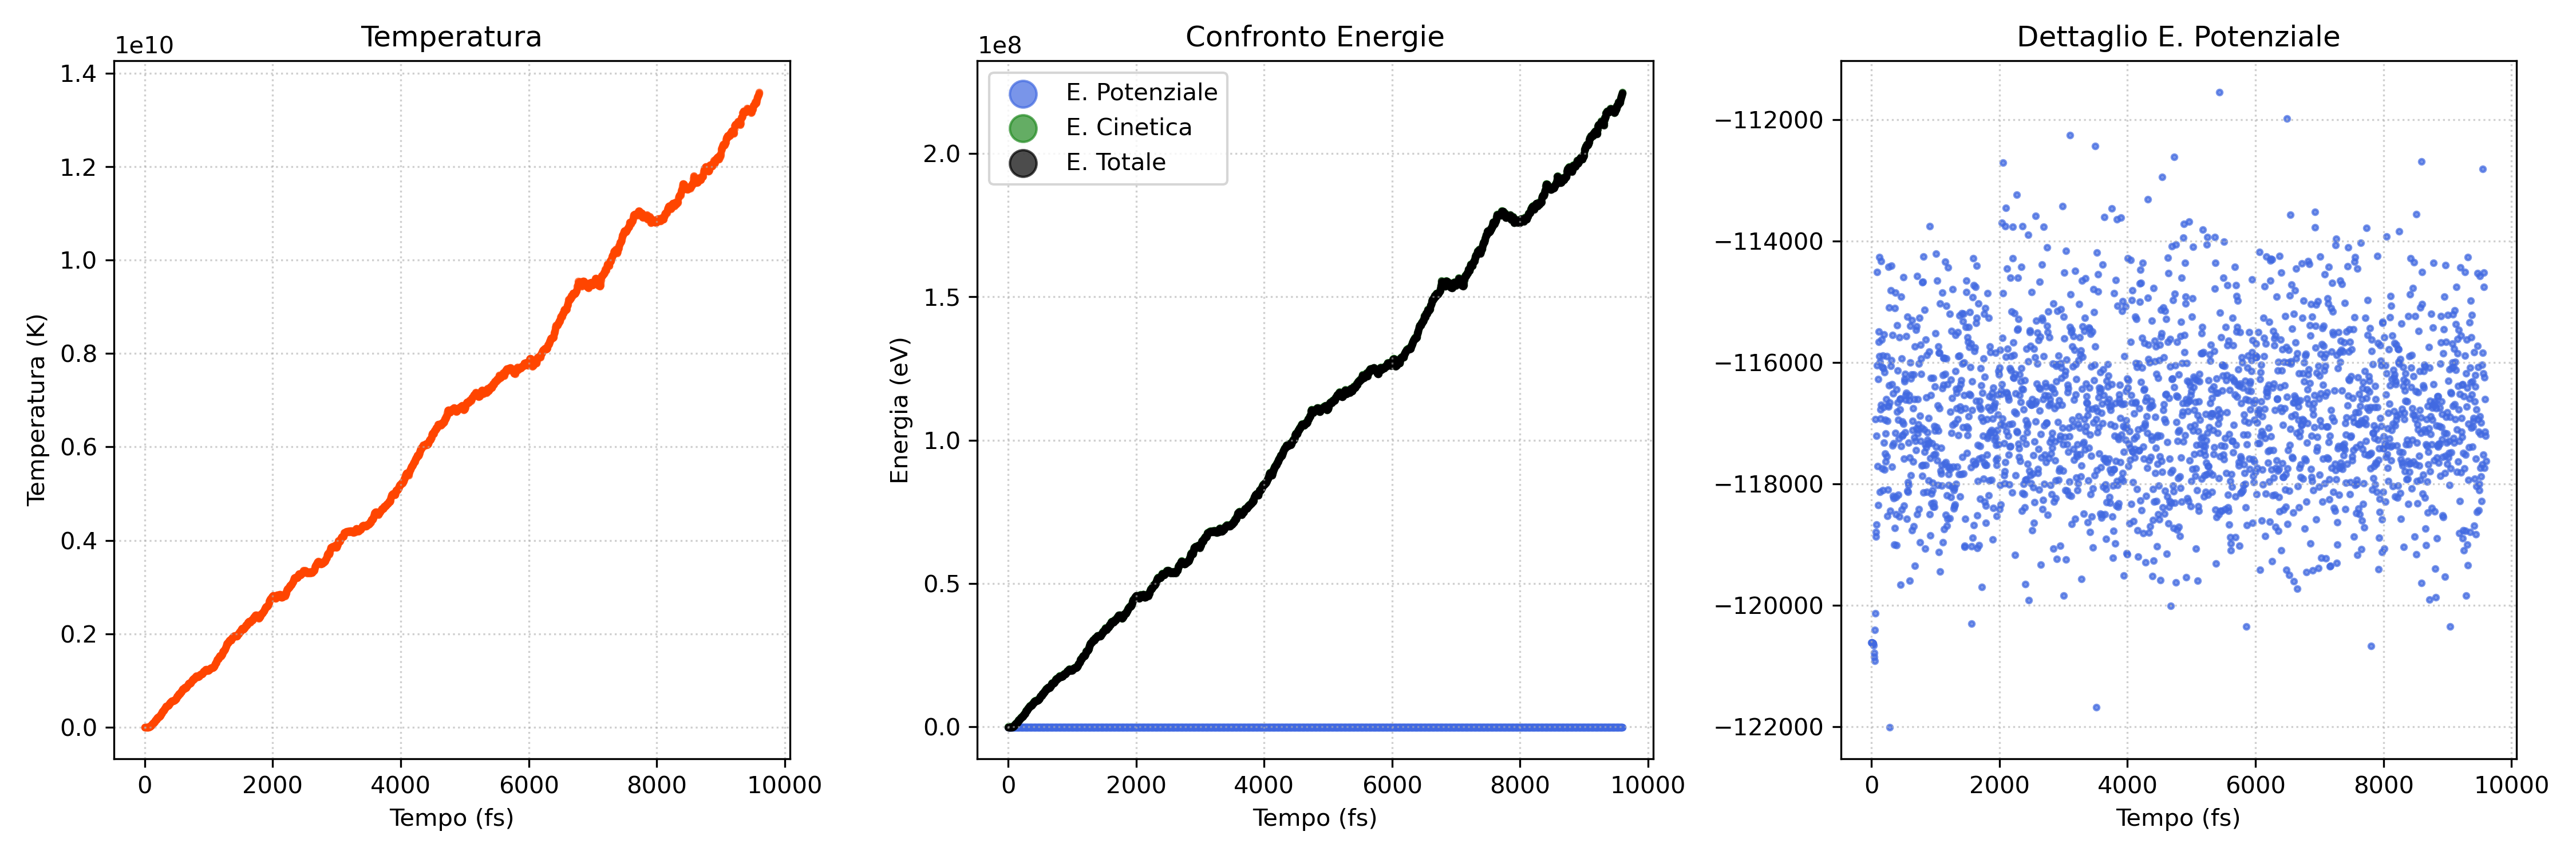
\includegraphics[scale=0.4]{./img/andamento_energia_nve_testdata.png}
    \caption{Grafico dell'andamento temporale per i valori di energia e temperatura.}
    \label{fig:andamento_nve-testdata}
\end{figure}

possiamo notare \ref{fig:andamento_nve-testdata} che i valori di energia e temperatura divergono a valori fisicamente insensati.
L'energia potenziale oscilla entro valori limite, notiamo comunque che l'intervallo di oscillazione è relativamente ampio.

Risulta utile anche guardare ai valori di forza associati a queste dinamica, riportati nel seguente grafico

\begin{figure}[h]
    \centering
    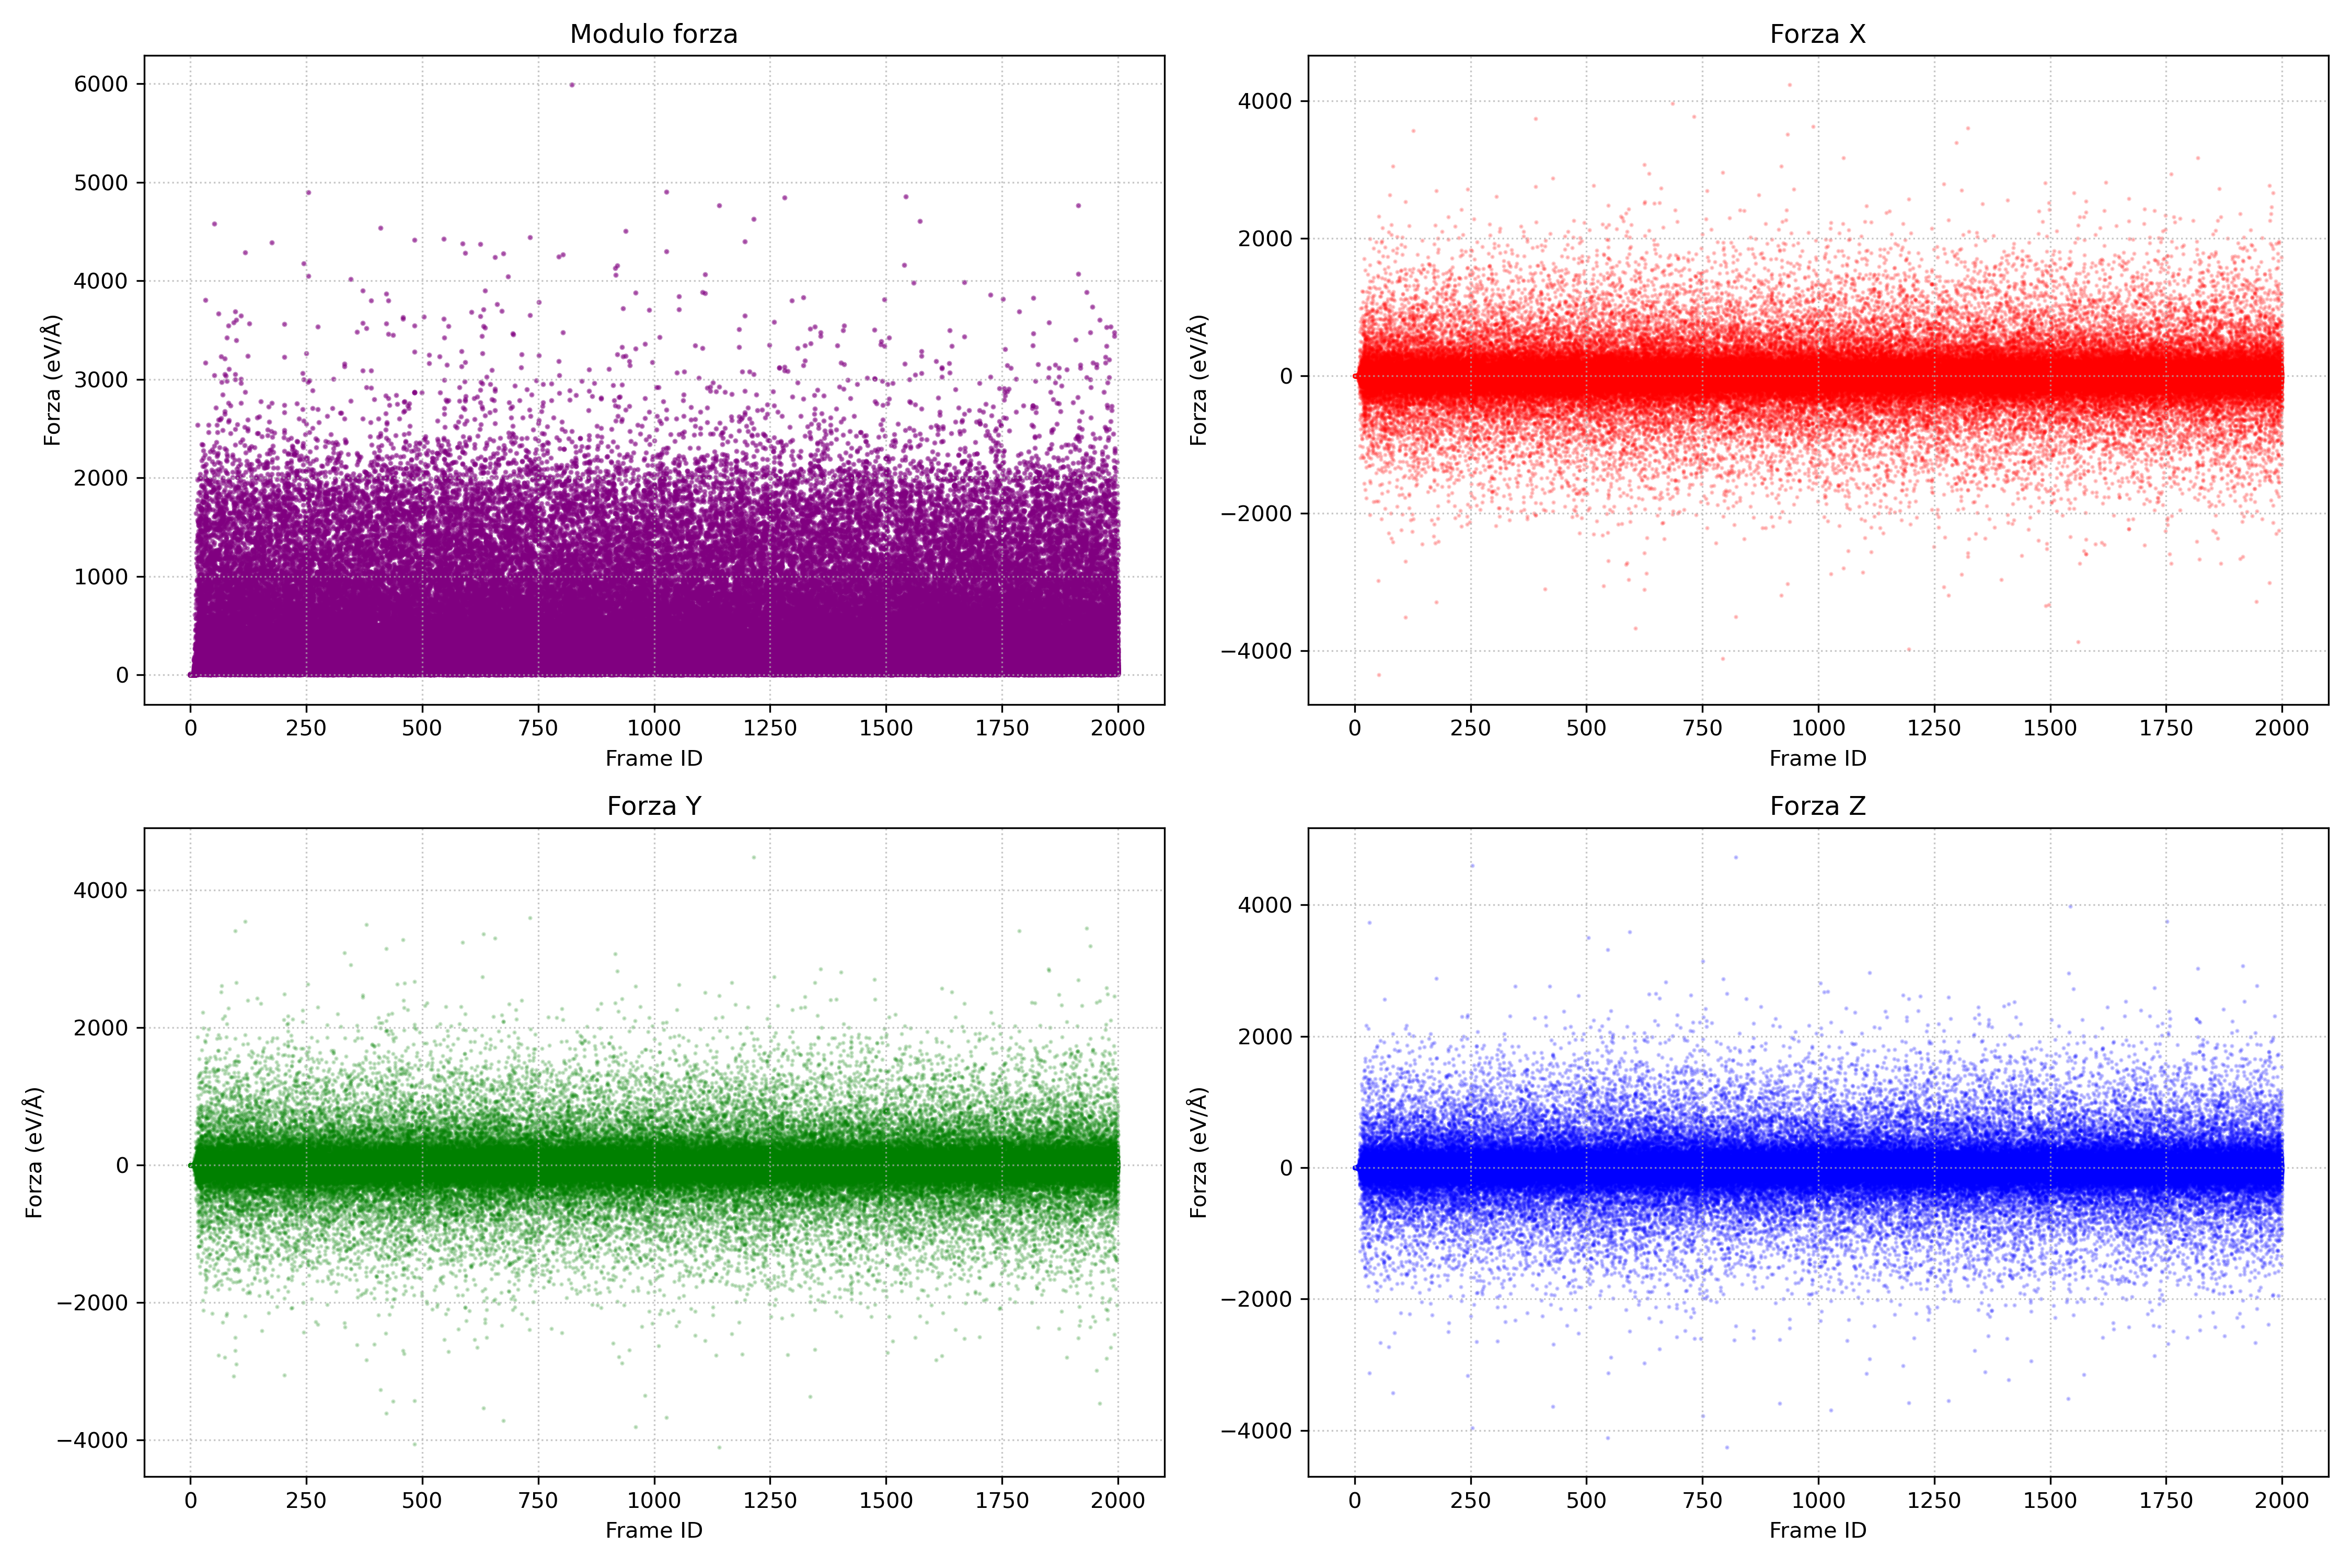
\includegraphics[scale=0.35]{./img/andamento_forze_totali_blocchi_nve_testdata.png}
    \caption{Grafico dell'andamento temporale per i valori di forza, sia in modulo che divise per componenti. }
    \label{fig:andamento_nve_forze-testdata}
\end{figure}

anche in questo caso possiamo notare che otteniamo valori estremamente elevati.



\section{Analisi delle problematiche} %--------------------------------------------------------------------------------------------------------------------------------------------------------------------------------------------------------

Abbiamo precedentemente menzionato che il potenziale è stato addestrato con parametri di soap non troppo elevati. Poniamo questo come ultimo problema da verificare in quanto i risultati sulle configurazioni di test erano discreti.
In questa sezioni ci poniamo di modificare a turno vari parametri, o combinazioni di tali, in modo da poter identificare quale sia il problema.


\subsection{Temperatura}

Come primo test abbiamo provato a modificare la temperatura dalla quale venivano estratti i valori di velocità. 
Si è impostato questo valore a $0$K, gli altri parametri sono rimasti invariati. 
Anche in questo caso diamo sia i riaultati per i valori di energia e temperatura

\begin{figure}[h]
    \centering
    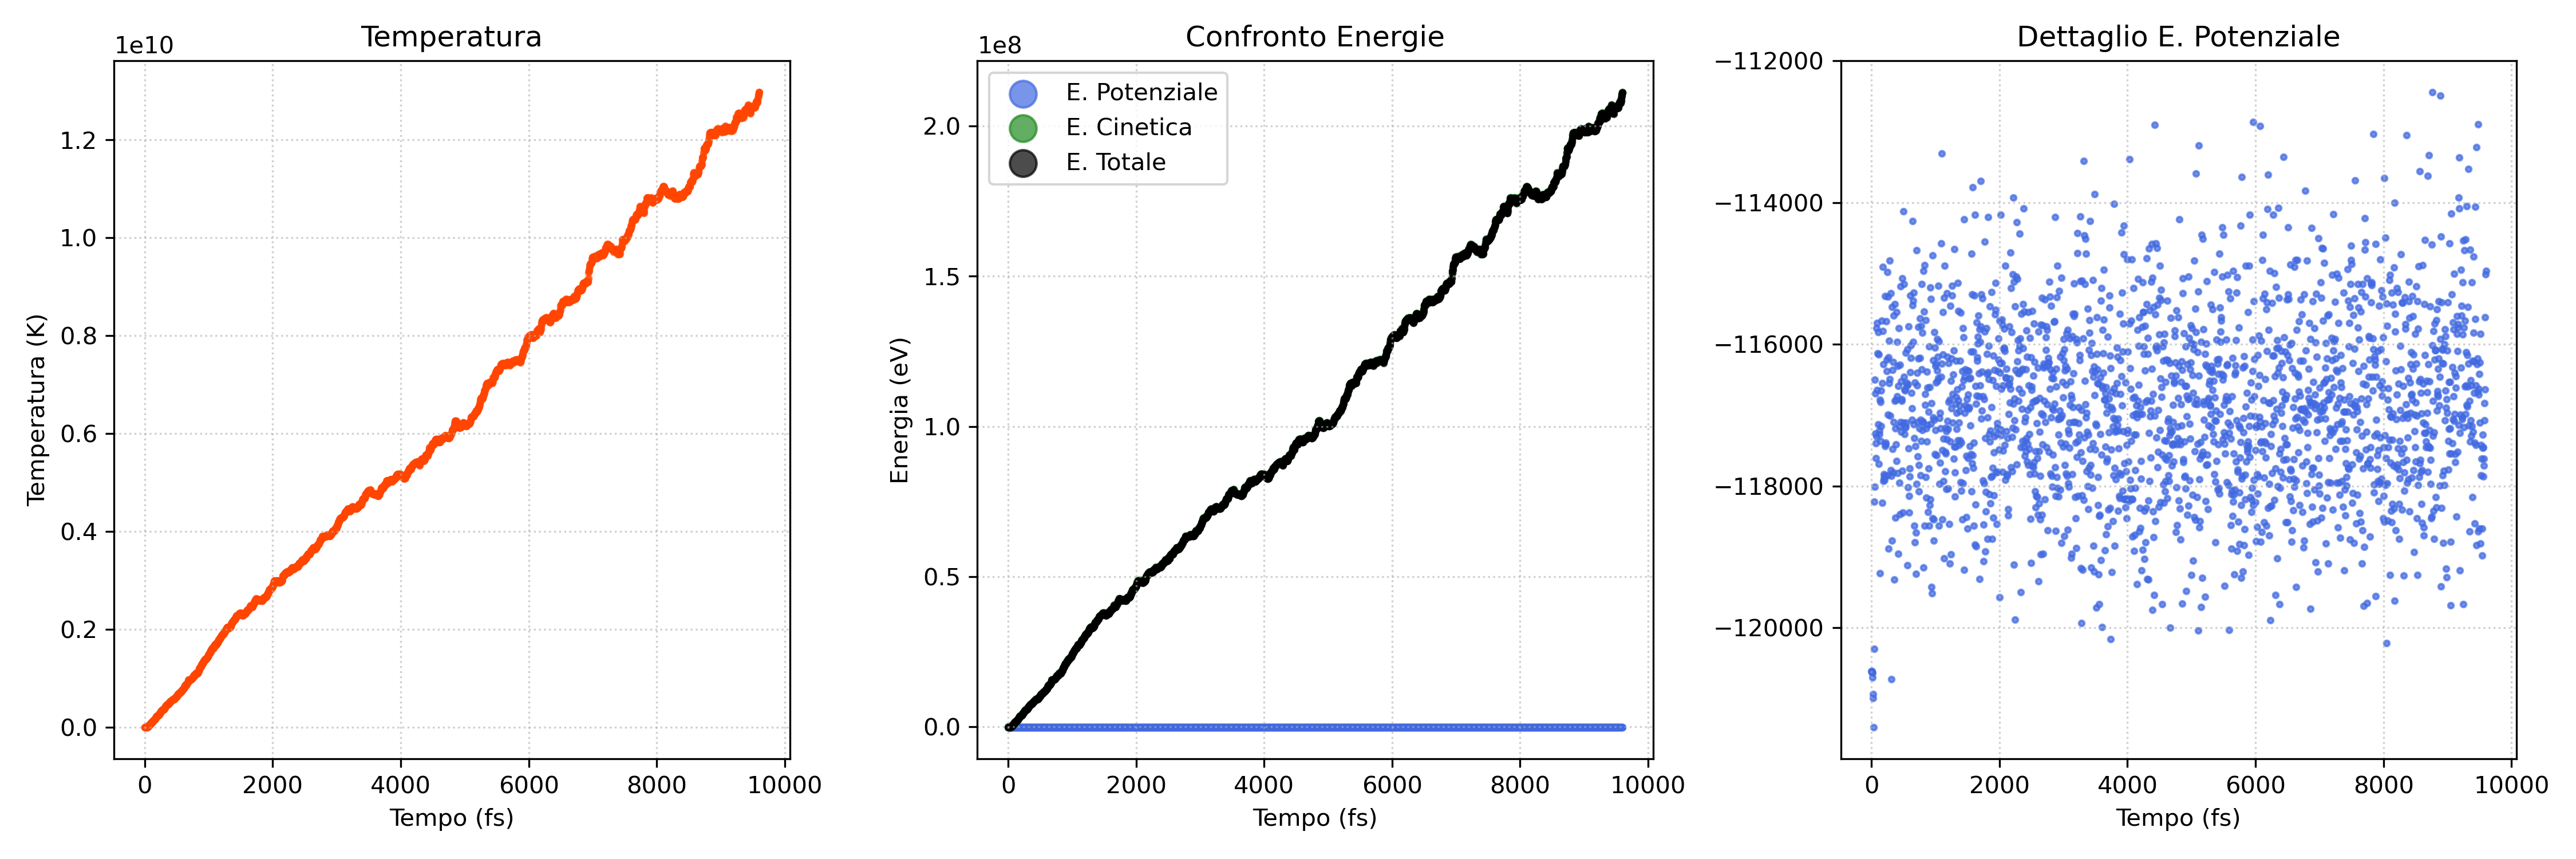
\includegraphics[scale=0.4]{./img/andamento_energia_nve_testdata_0k.png}
    \caption{Grafico dell'andamento temporale per i valori di energia e temperatura}
    \label{fig:andamento_nve-traindata_0k}
\end{figure}

che per i valori delle forze

\begin{figure}[h]
    \centering
    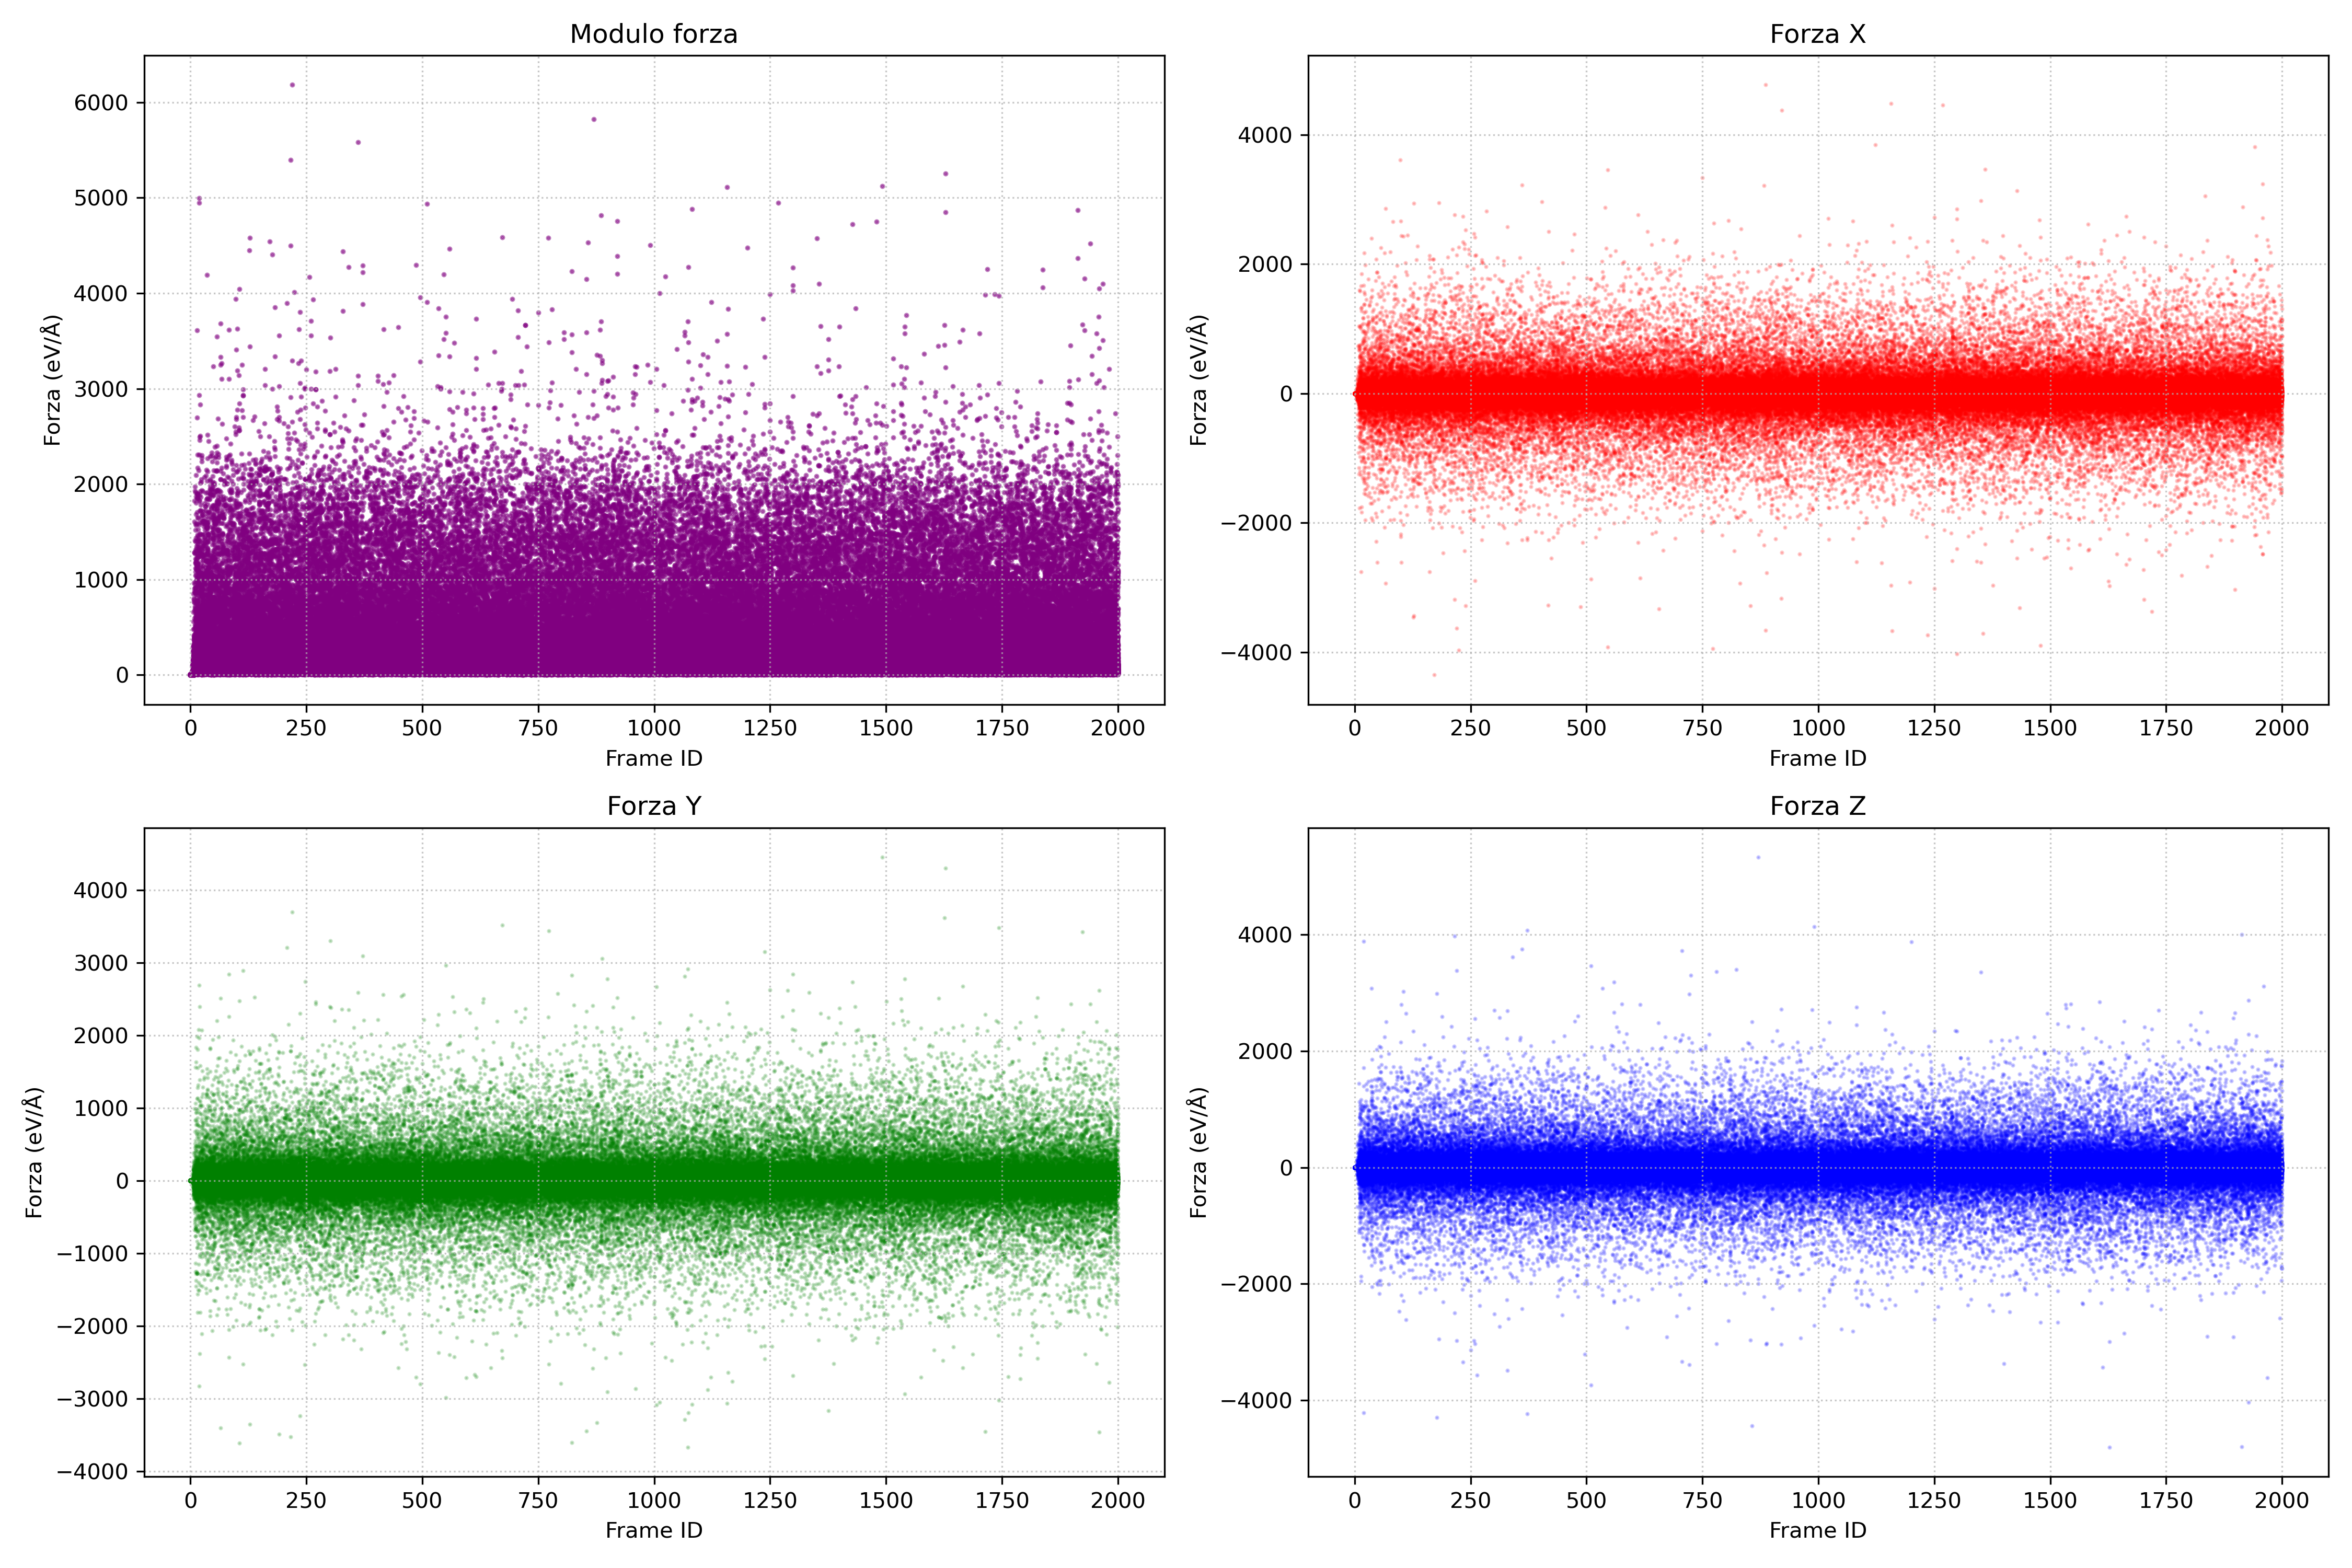
\includegraphics[scale=0.35]{./img/andamento_forze_totali_blocchi_nve_testdata_0k.png}
    \caption{Grafico dell'andamento temporale per i valori di forza, sia in modulo che divise per componenti. }
    \label{fig:andamento_nve_forze-traindata_0k}
\end{figure}

Si nota \ref{fig:andamento_nve-traindata_0k} e \ref{fig:andamento_nve_forze-traindata_0k} che il risultato non è dissimile da quello ottenuto in precedenza, possiamo quindi escludere che sia un problema legato al valore di temperatura.



\subsection{Timestep} %----------------------------------------------------------------------------------------------------------------------------------------------------------------------------------------------------------------------

Per questa analisi sono stati provati diversi valori di timestep, riportiamo solo uno di questi.
Come timestep si è impostato un valori di $10^{-5}$fs, e un totale di $50'000$ iterazioni, in modo da valutate la stabilità sul lungo periodo. Si è mantenuta una temperatura di $3'000$K.

I valori di energia e temperatura sono rappresentati nel seguente grafico \ref{fig:andamento_nve_energie_timestep}

\begin{figure}[h]
    \centering
    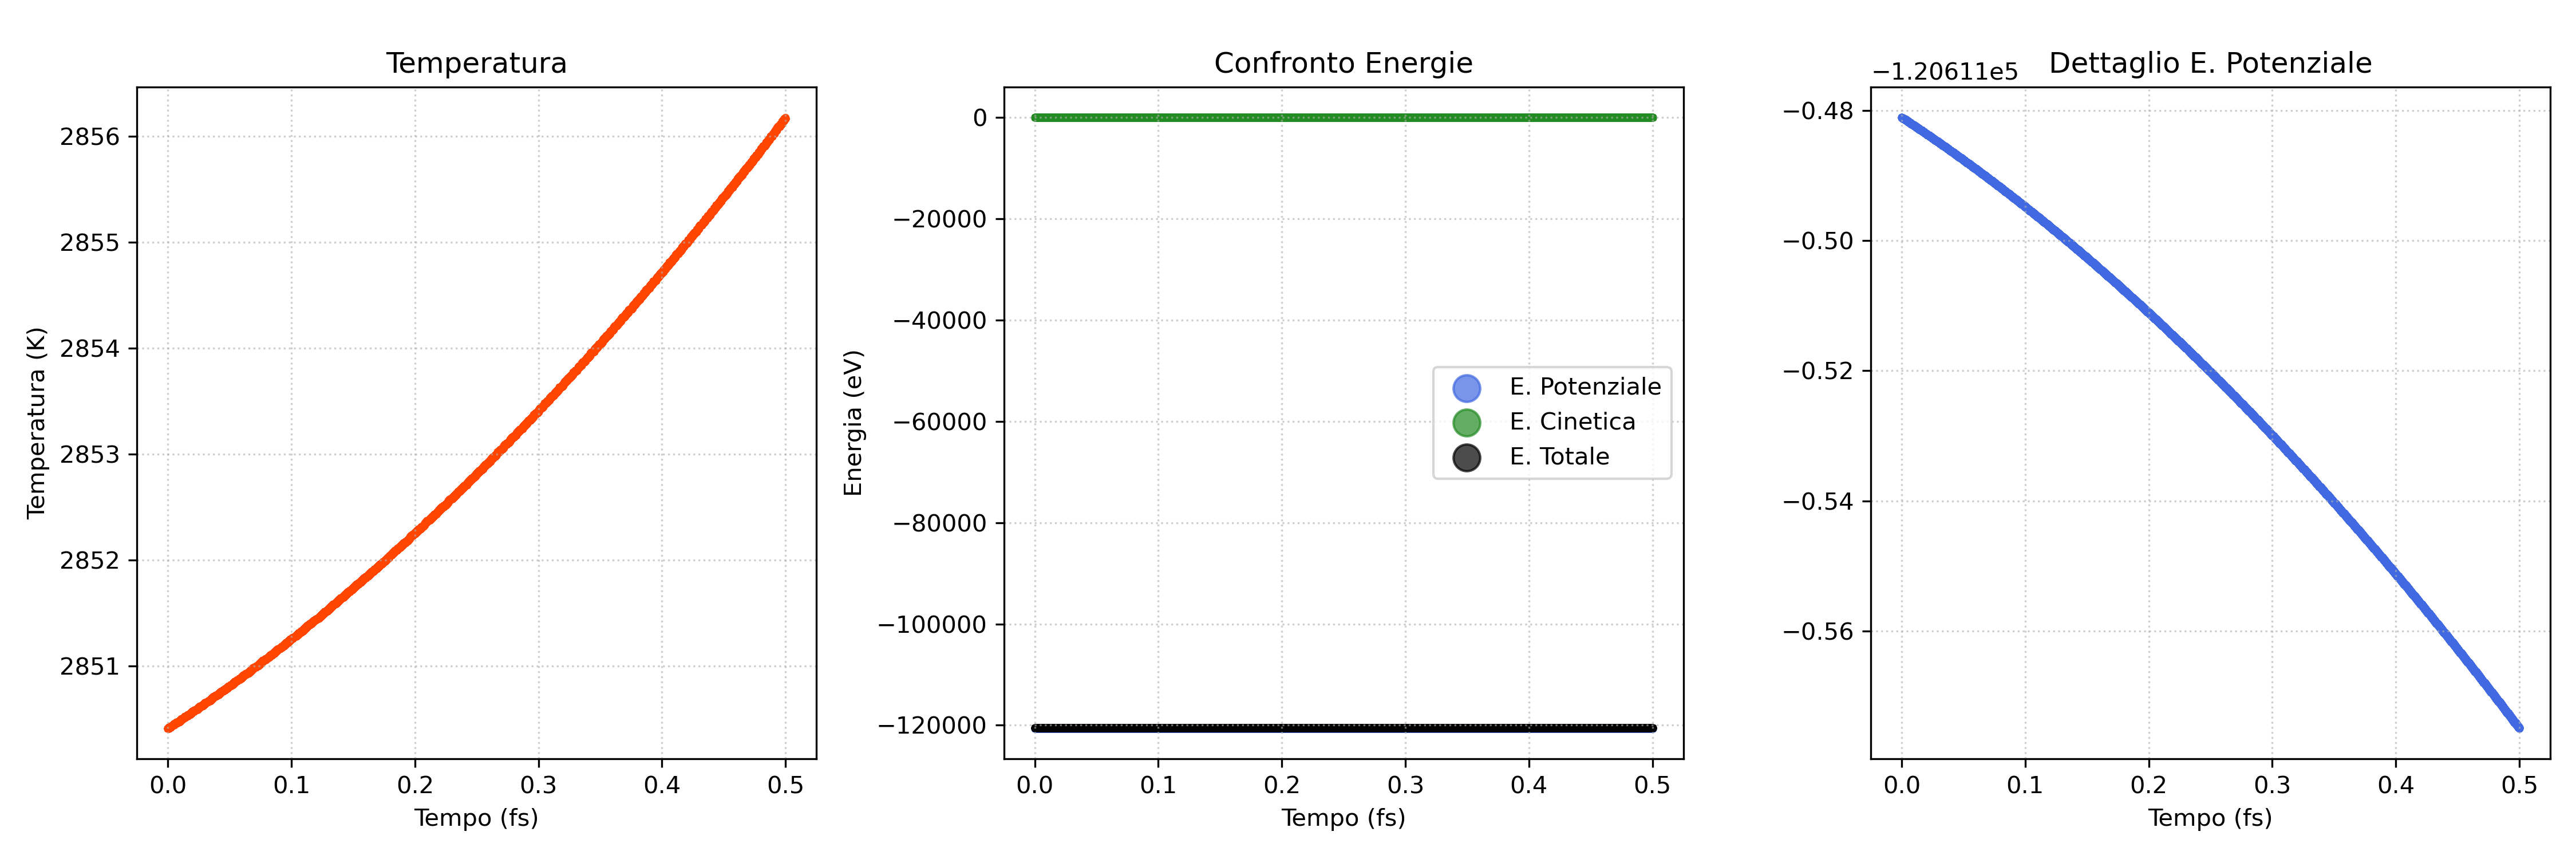
\includegraphics[scale=0.4]{./img/andamento_energia_nve_timestep.png}
    \caption{Grafico dell'andamento temporale per i valori di energia e temperatura}
    \label{fig:andamento_nve_energie_timestep}
\end{figure}

mentre per quanto riguarda le forze otteniamo il grafico \ref{fig:andamento_nve_forze_timestep}


\begin{figure}[h]
    \centering
    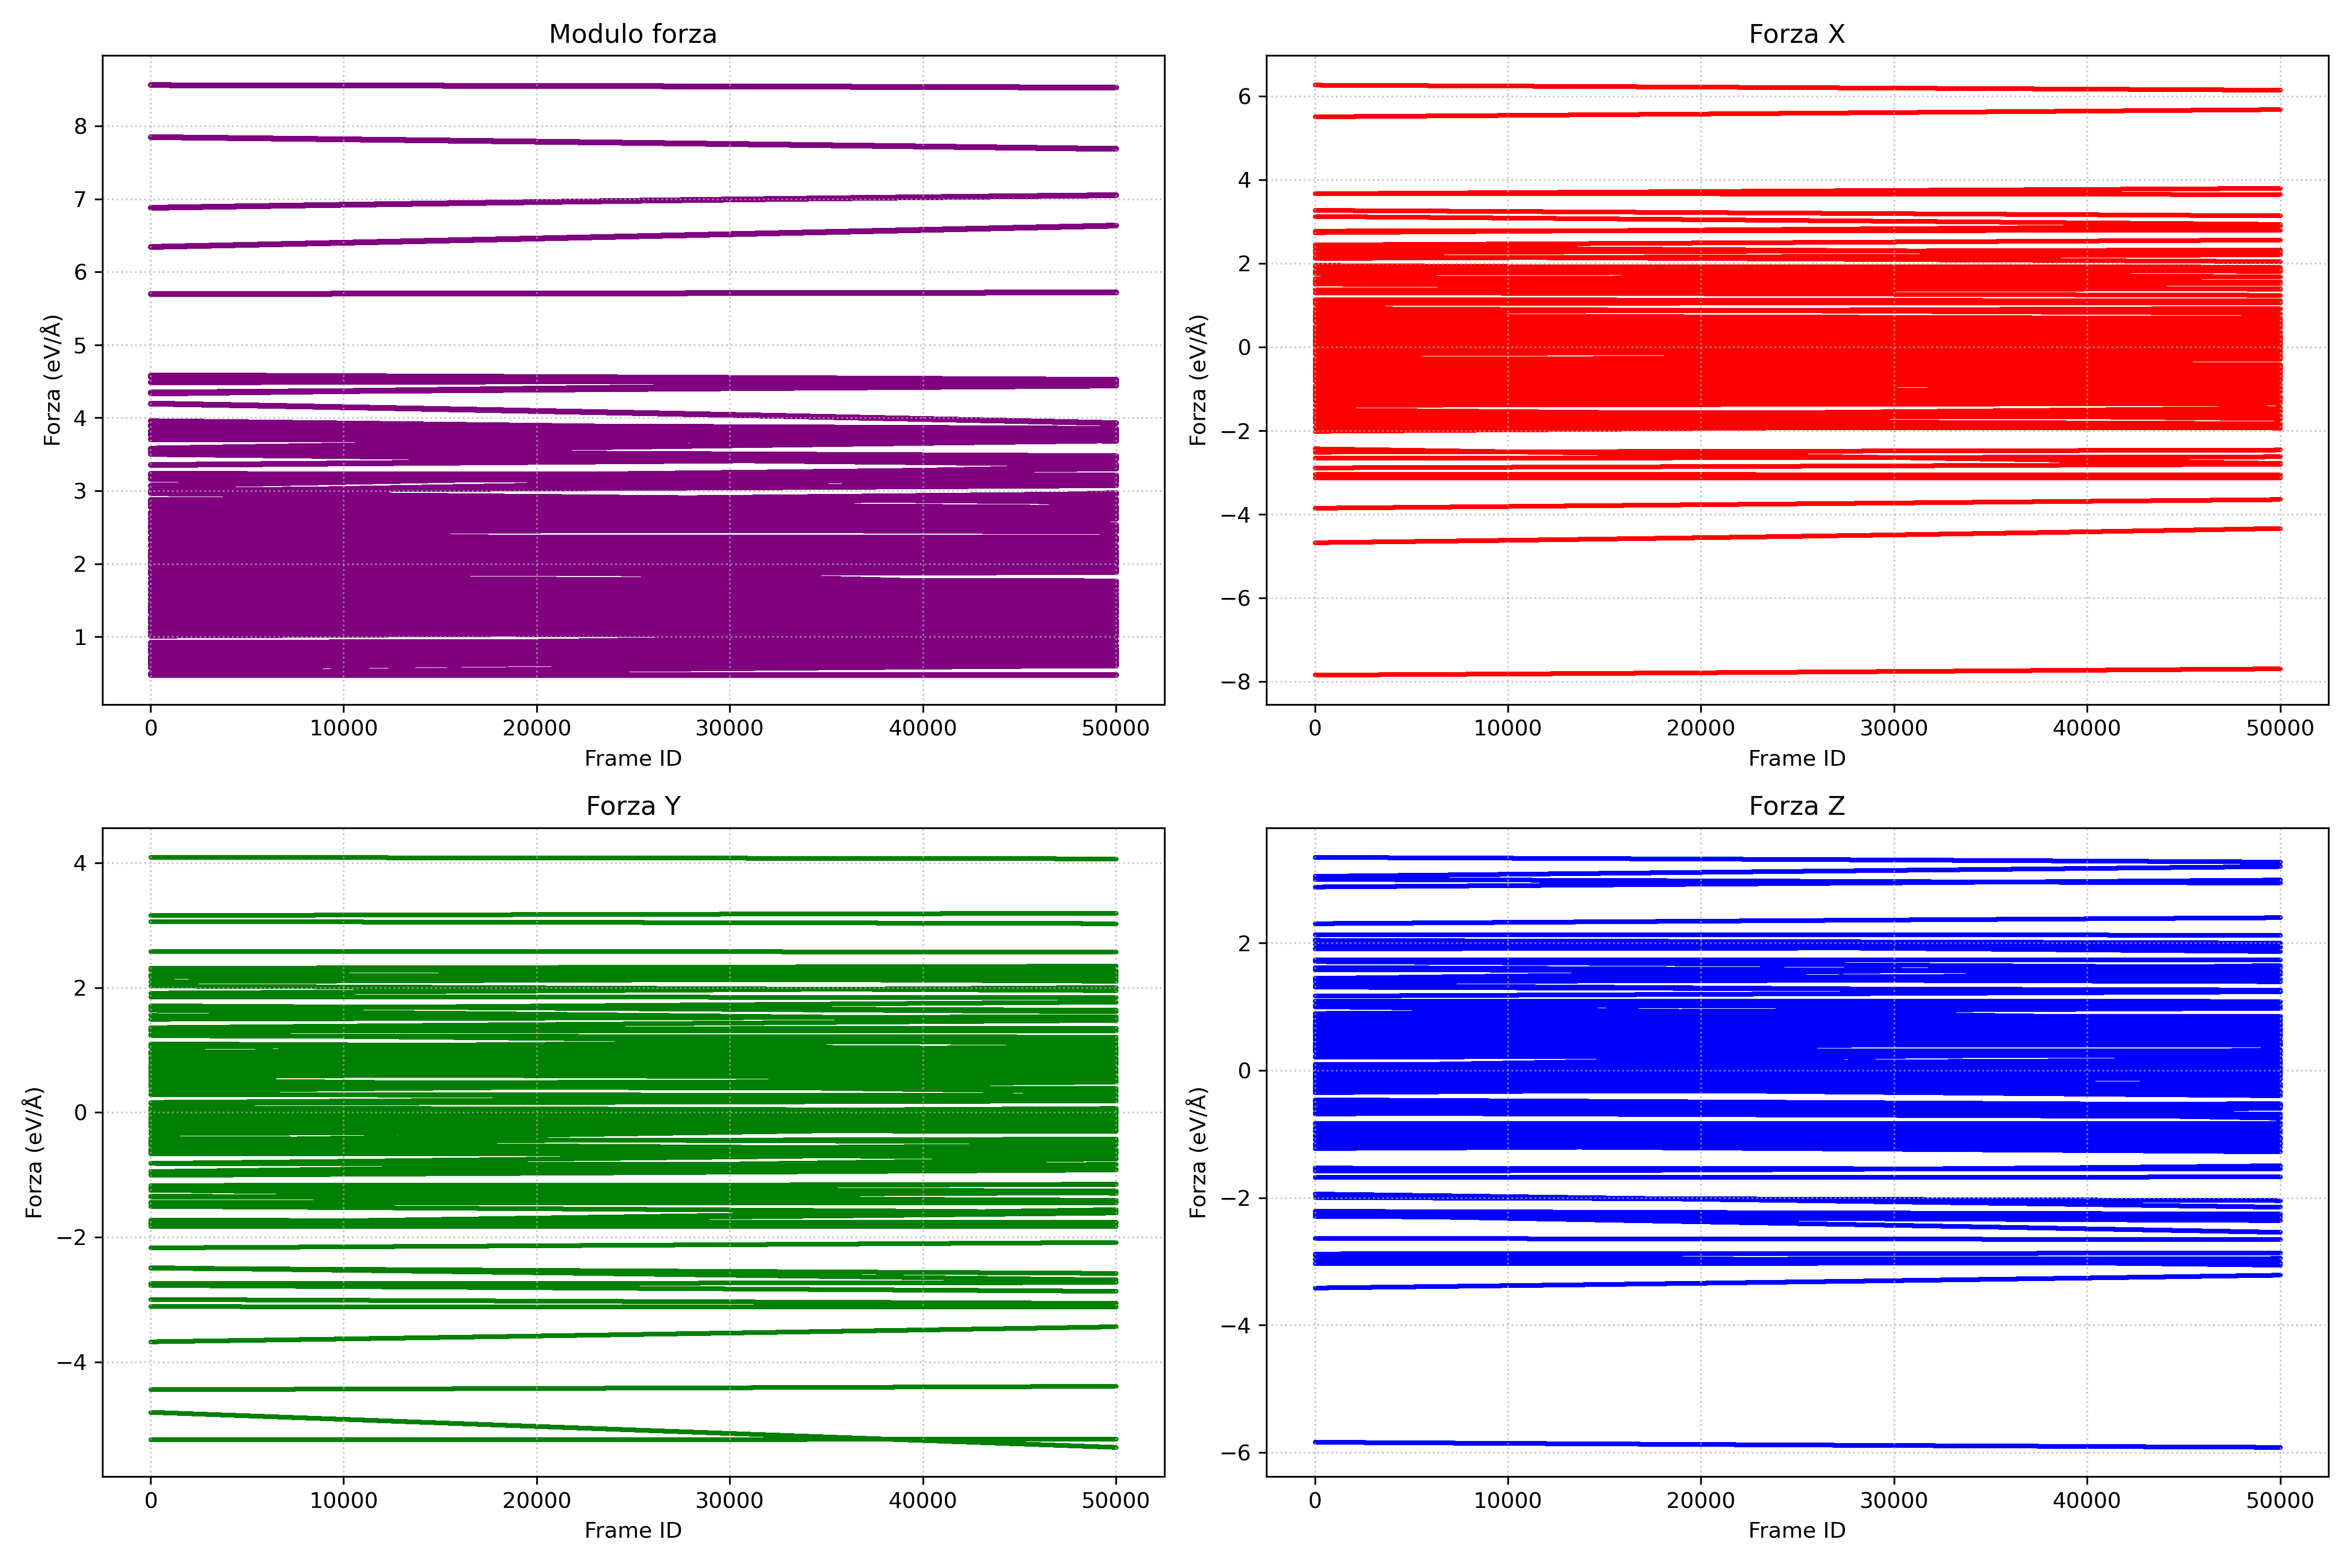
\includegraphics[scale=0.35]{./img/andamento_forze_totali_blocchi_nve_timestep.png}
    \caption{Grafico dell'andamento temporale per i valori di energia e temperatura}
    \label{fig:andamento_nve_forze_timestep}
\end{figure}


considerando questo risultato \ref{fig:andamento_nve_energie_timestep} la prima cosa che si vede è una diminuzione del range in cui i valori di temperatura e di energia variano.
Ad ogni modo possiamo notare che entrambe mantengono la medesima forma vista in precedenza, possiamo quindi presumere che stiano comunque divergendo, ma ad un rate estremamente basso.
Anche i valori delle forze sono contenuti.
Considerando la tipologia di integratore numerico utilizzato in questa simulazione, questo risultato era prevedibile.


\subsection{Distanze e forze}

Risulta utile andare a guardare la distribuzione dei valori delle distanze tra i primi vicini, per ogni frame si prente come atomo il $j$-esimo e se ne calcola la distanza con i restanti 125, se ne prende poi il minimo, questo per ogni atomo presente nel frame. Successivamente guardiamo la relazione tra i valori di distanza e i valori di forza.

Nei grafici a due pannelli successivi vogliamo evidenziare queste relazioni.

Per il caso del semplice potenziale GAP, come notiamo nella figura (\ref{fig:confronto_forze_distanze_gap_testdata})

{
\begin{figure}[ht]
    \centering

    \begin{subfigure}{0.48\textwidth}
        \centering
        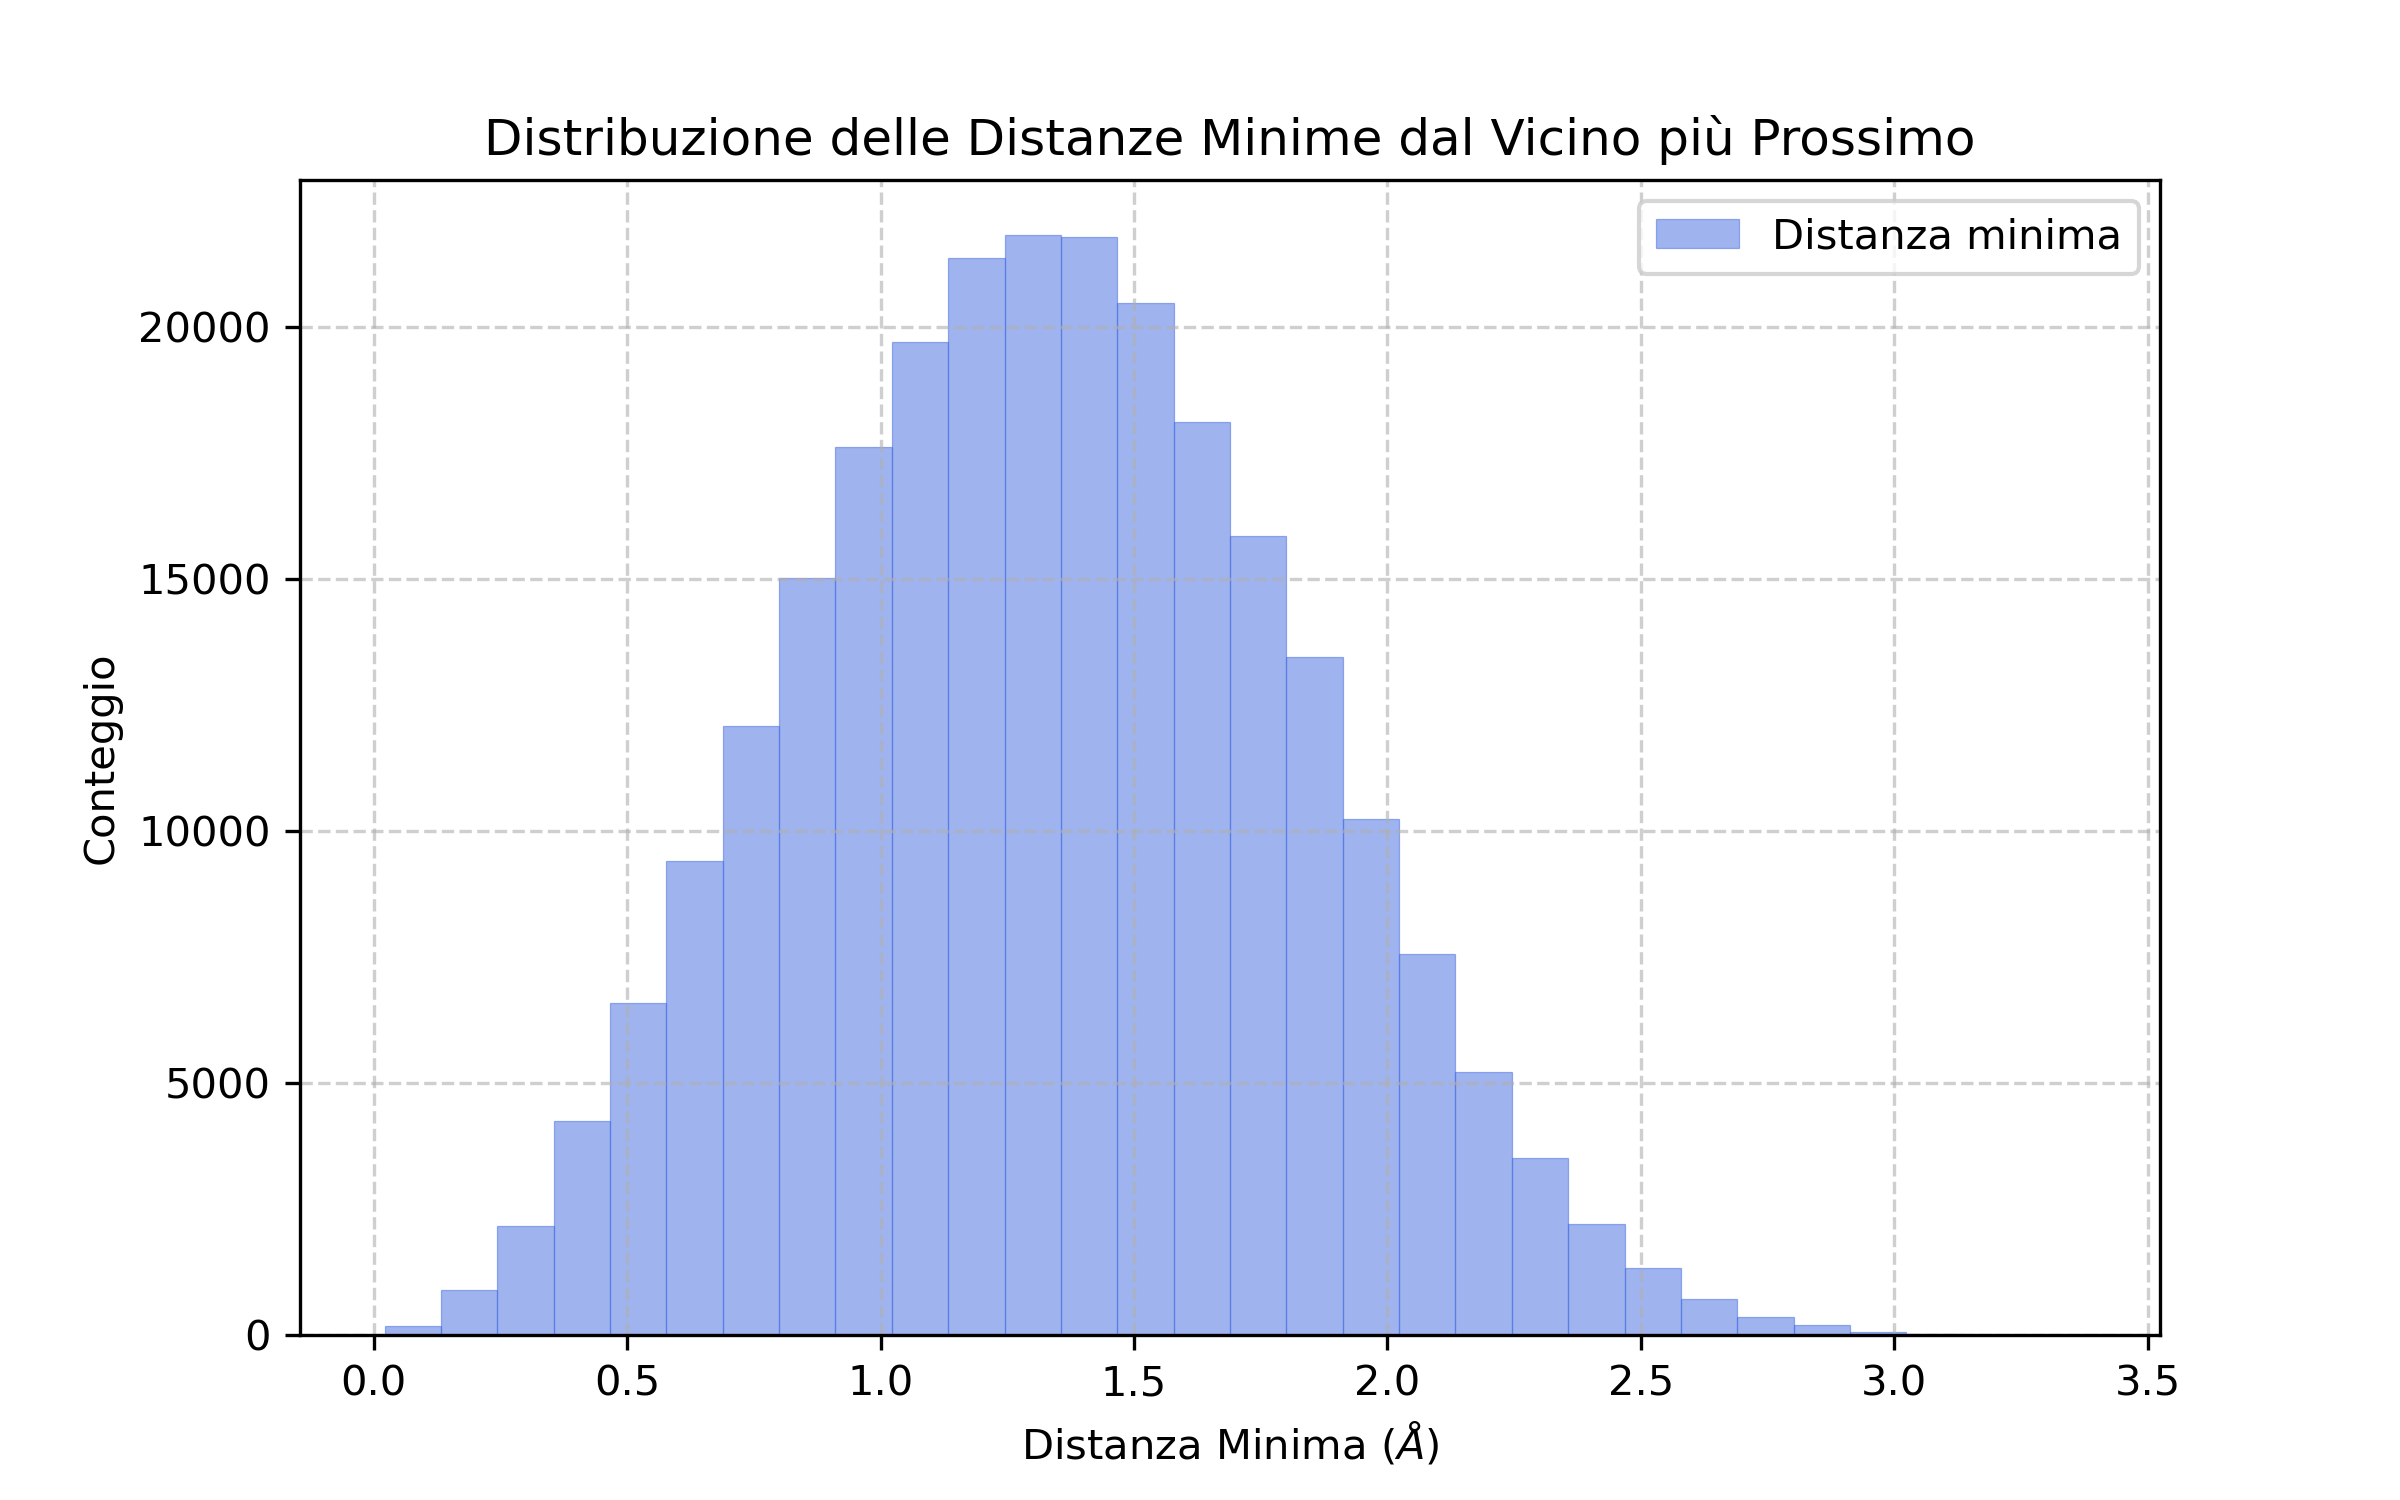
\includegraphics[width=\linewidth]{./img/histo_distanze_nve_testdata.png}
        \caption{Istogramma dei valori di distanza tra i primi vicini per il solo potenziale GAP}
    \end{subfigure}
    \hfill
    \begin{subfigure}{0.48\textwidth}
        \centering
        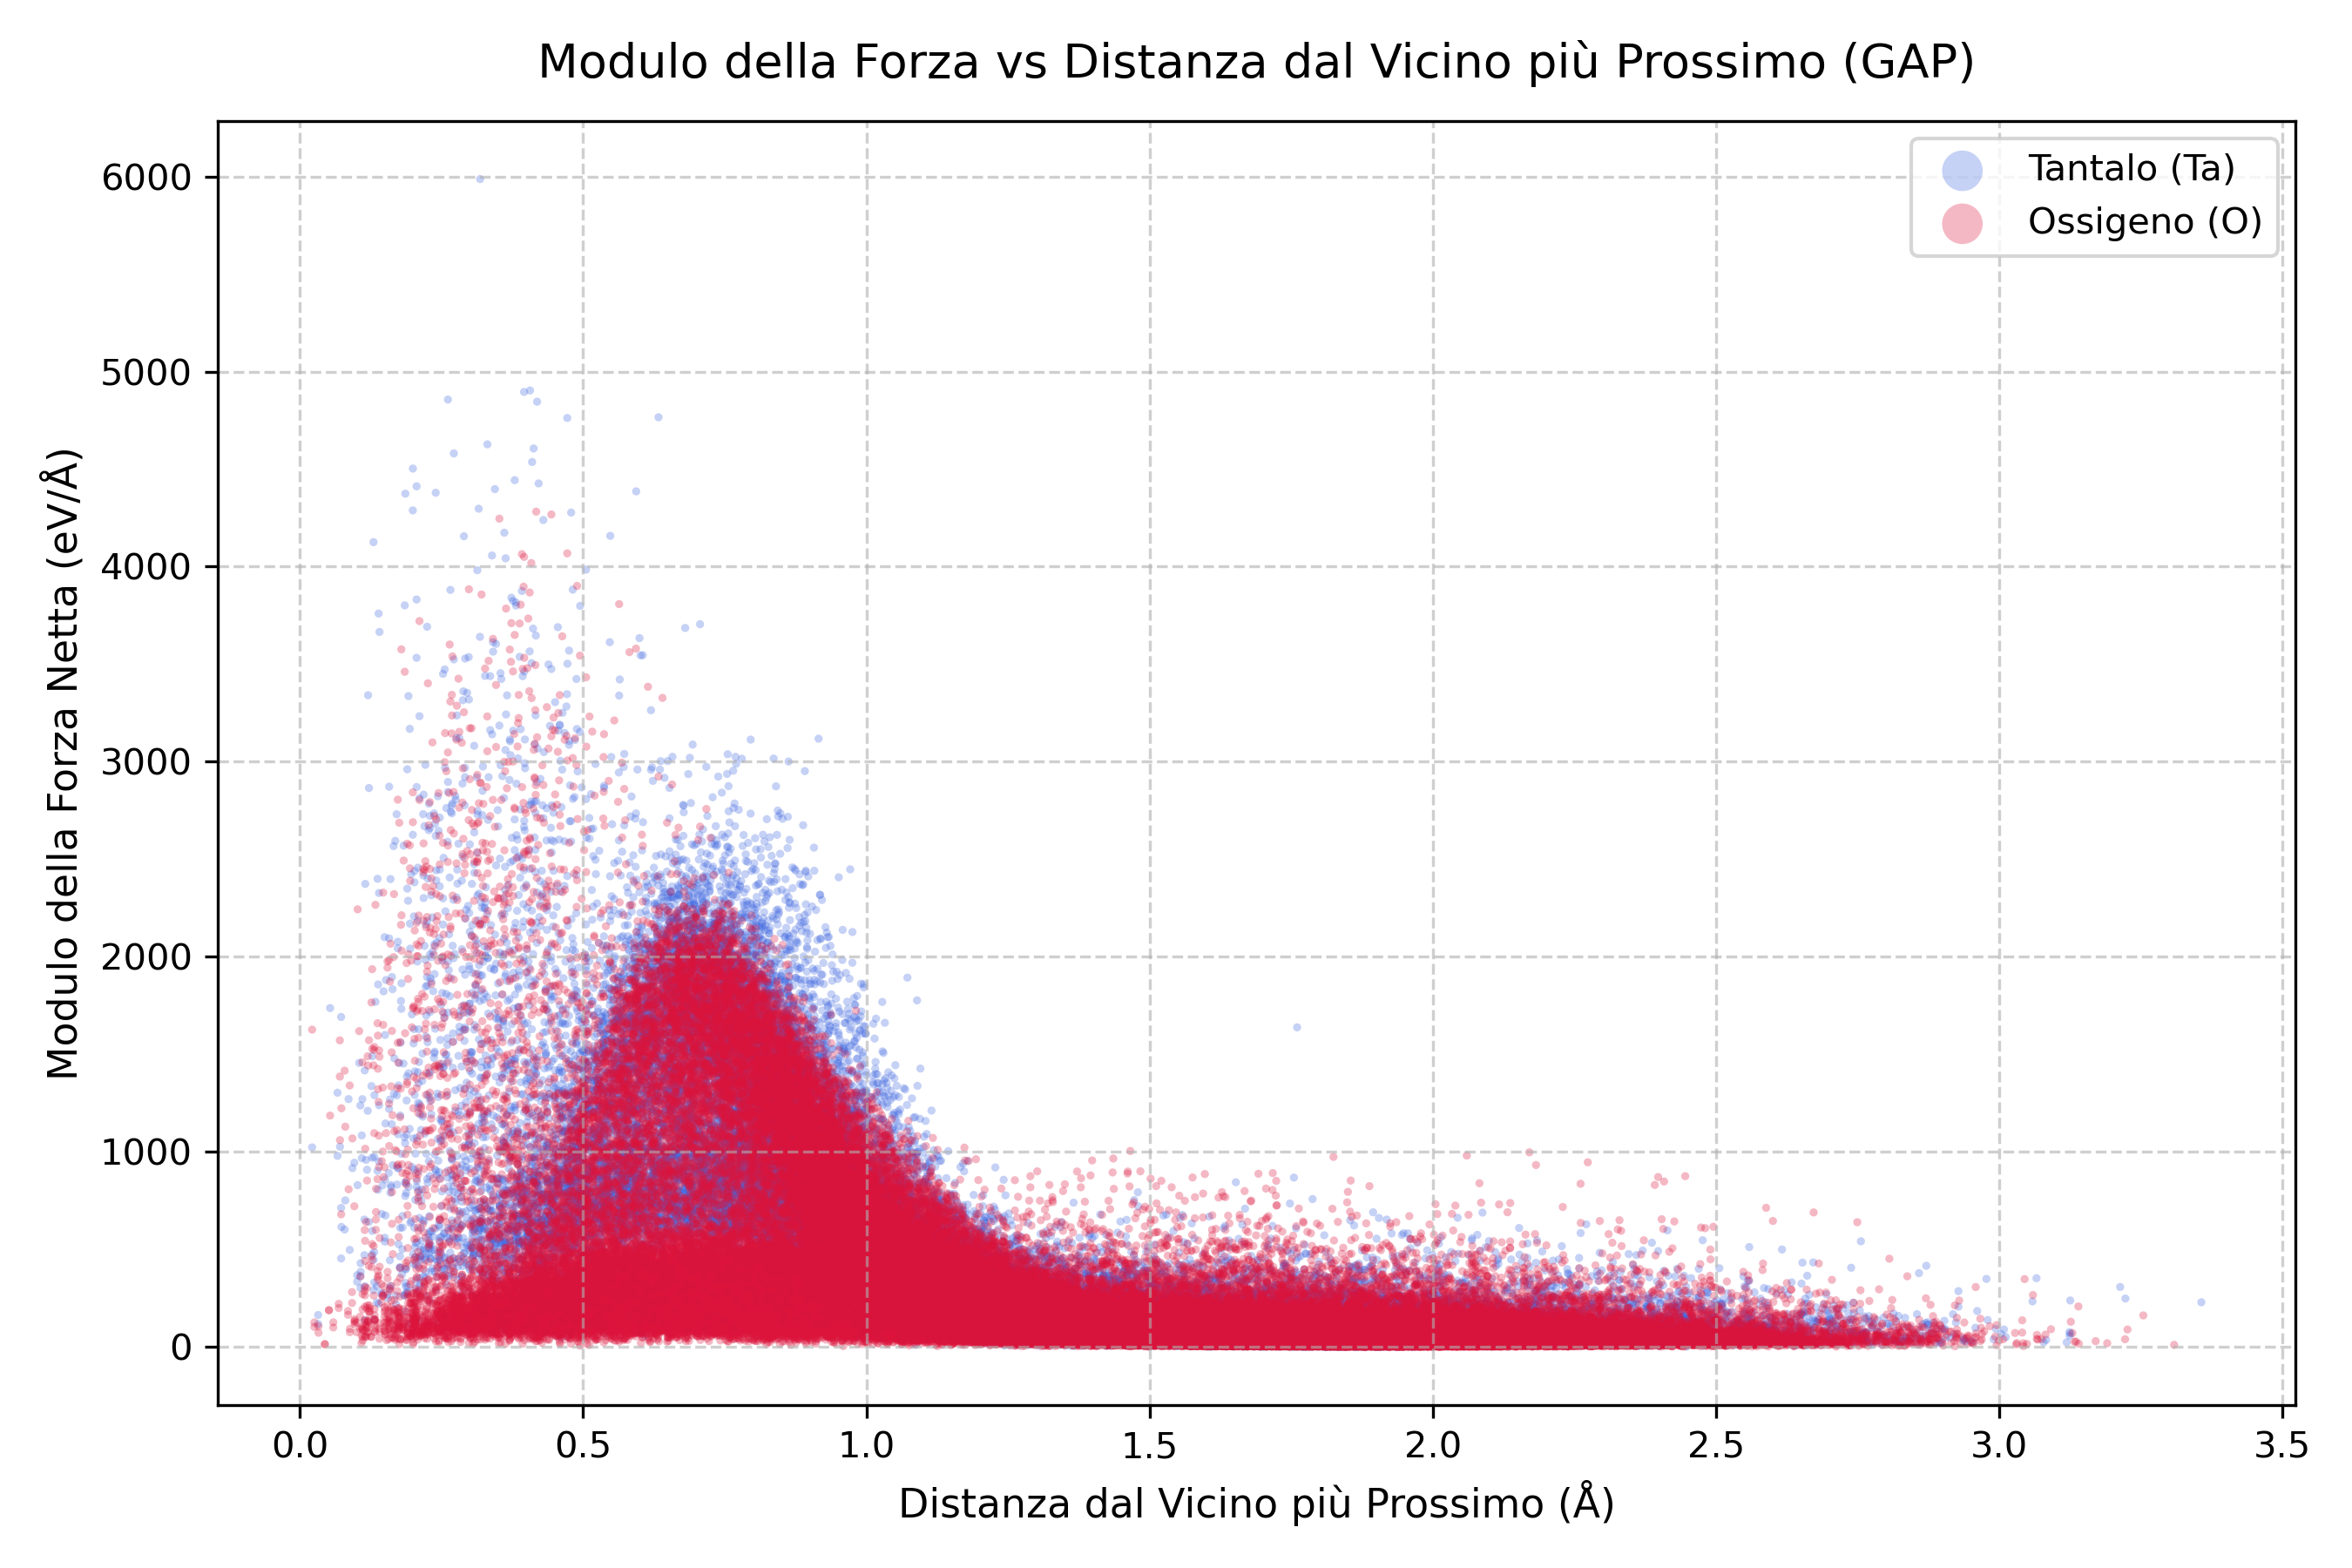
\includegraphics[width=\linewidth]{./img/andamento_forze_totali_distanza_nve_testdata.png}
        \caption{Relazione tra i valori di forza e distanza tra i primi vicini}
    \end{subfigure}

    \caption{Distanze e relazione forze distanze per il caso del solo potenziale GAP}
    \label{fig:confronto_forze_distanze_gap_testdata}
\end{figure}
}

la maggior parte dei valori di distanza si trova al di sotto del valore di $1.5$\AA. 
Si vede facilmente dove le forze assumono il loro valore maggiore.

Questo diventa rilevante nel momento in cui andiamo ad analizzare i valori di distanza tra i primi vicini e le relative forze, calcolati nel medesimo modo, presenti nelle configurazioni utilizzate nella fase di training, queste sono riportate in figura (\ref{fig:confronto_forze_distanze_qe_traindata})

{
\begin{figure}[ht]
    \centering

    \begin{subfigure}{0.48\textwidth}
        \centering
        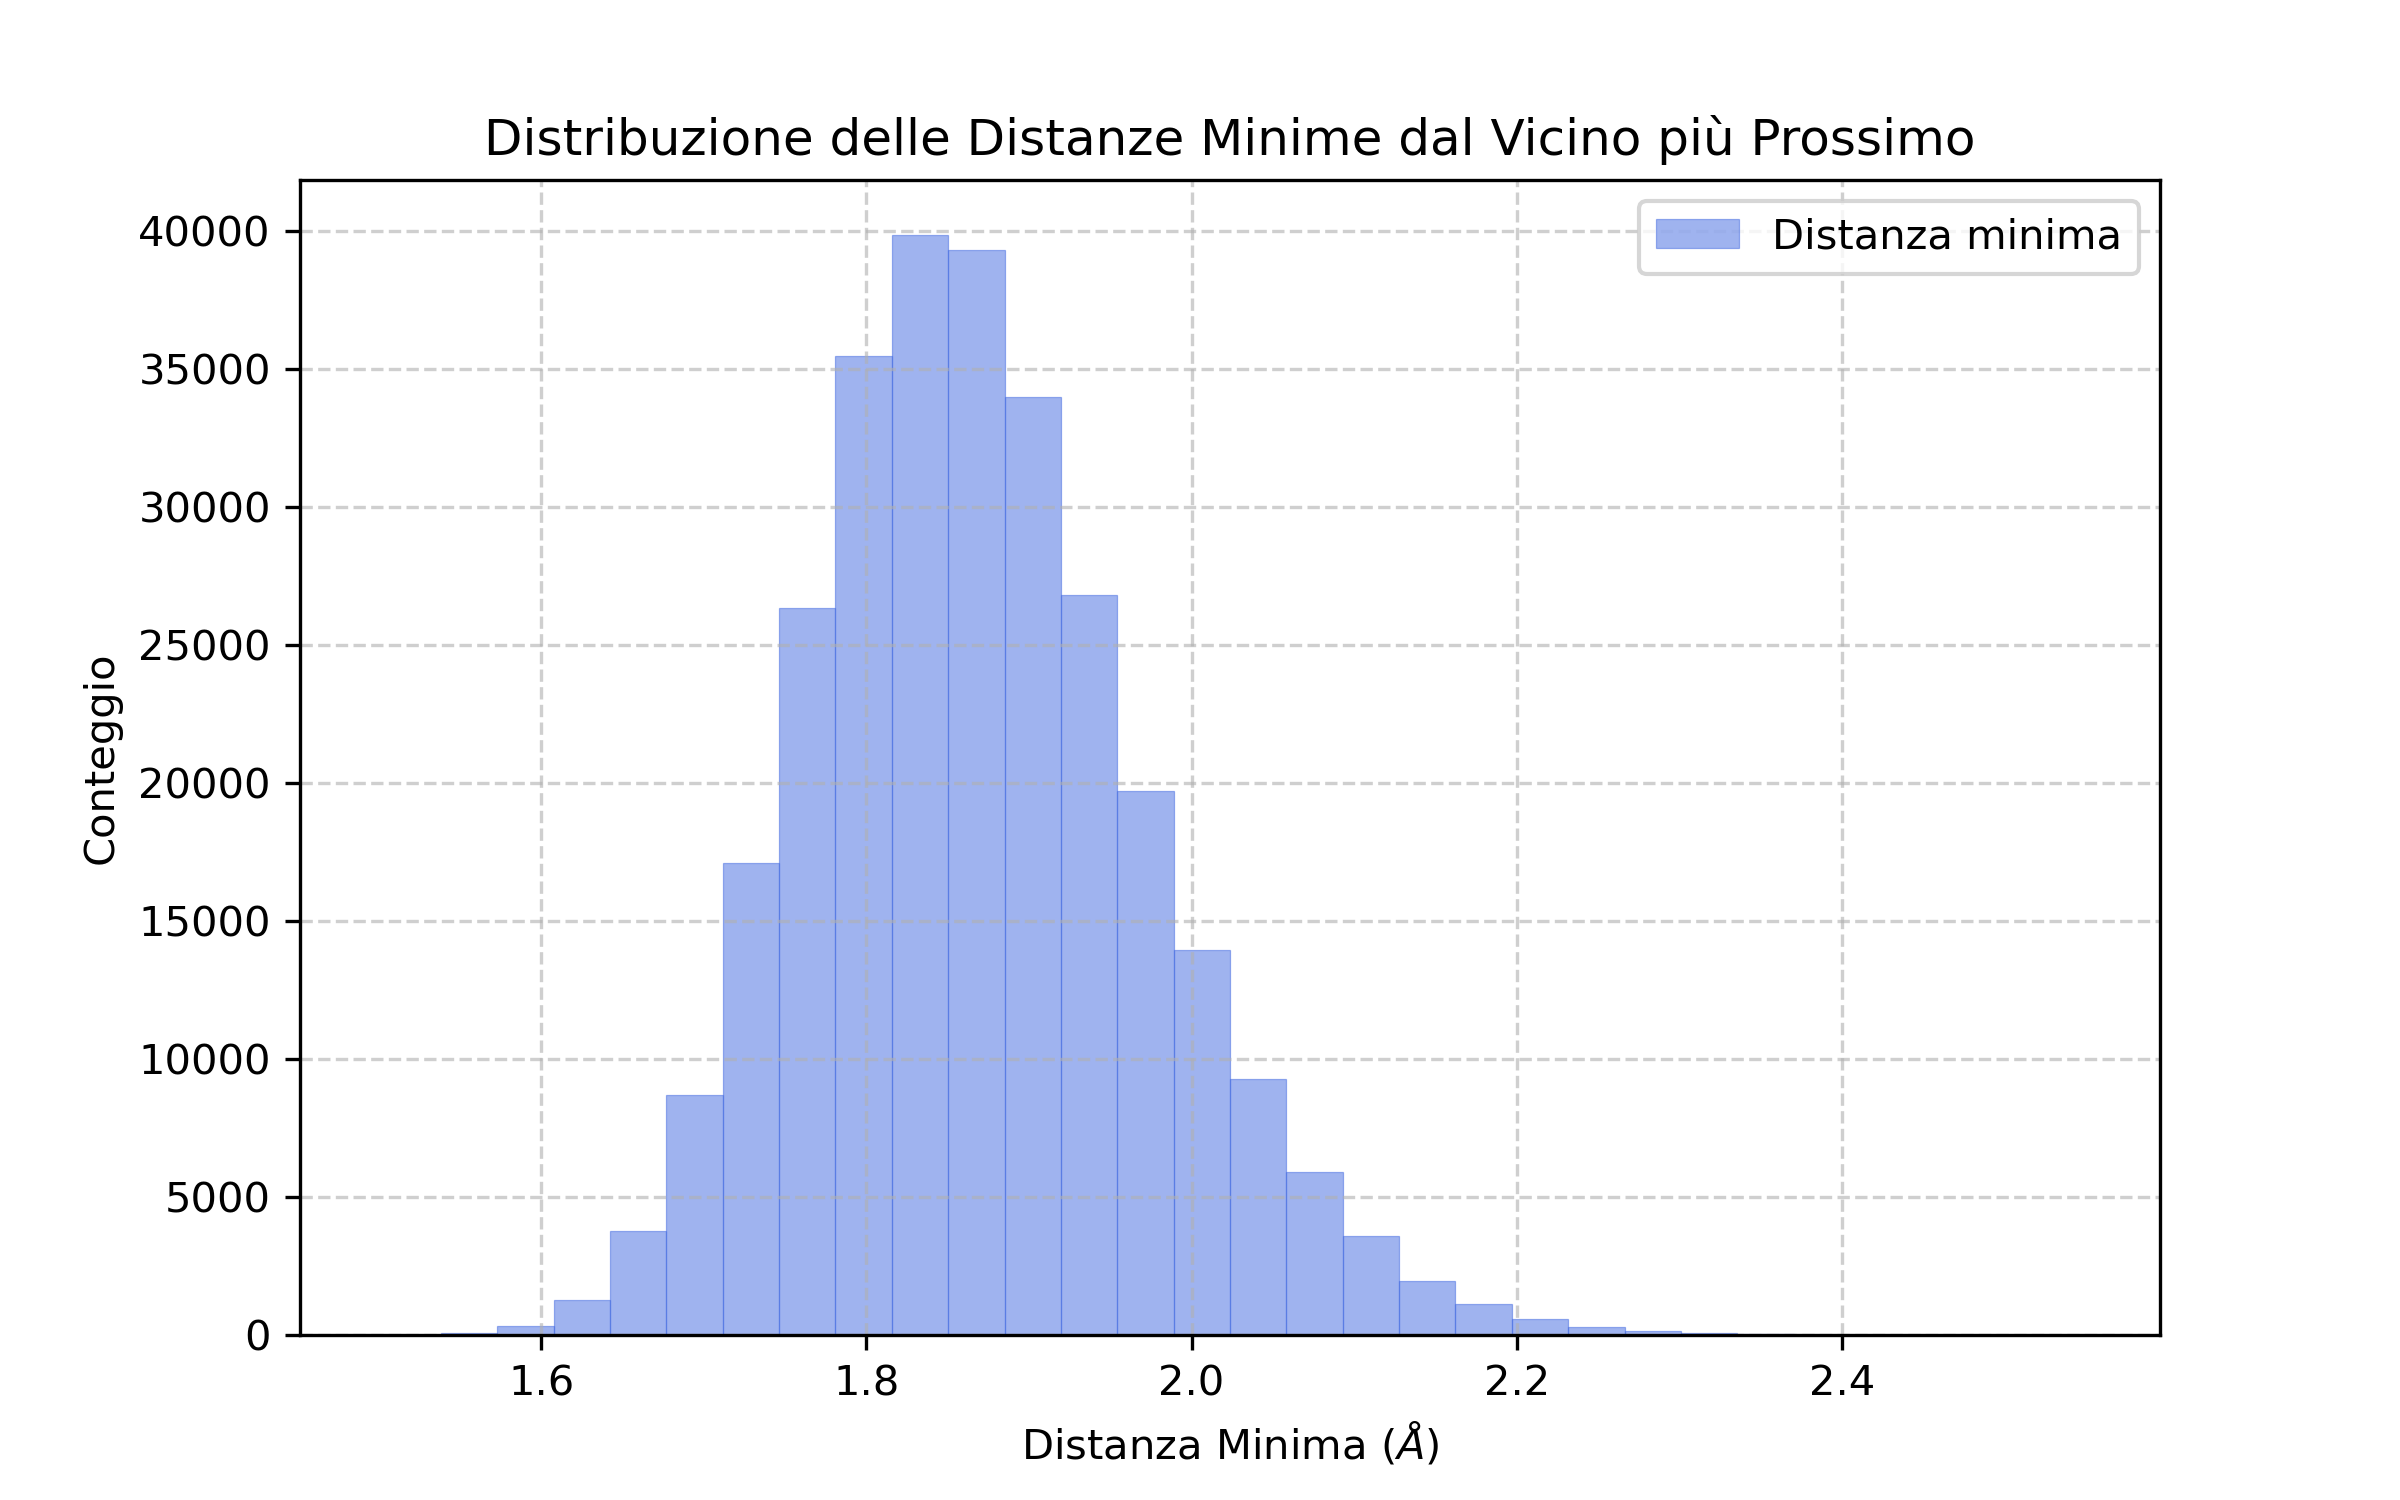
\includegraphics[width=\linewidth]{./img/histo_distanze_qe_traindata.png}
        \caption{Istogramma dei valori di distanza tra i primi vicini per il set di dati di training}
    \end{subfigure}
    \hfill
    \begin{subfigure}{0.48\textwidth}
        \centering
        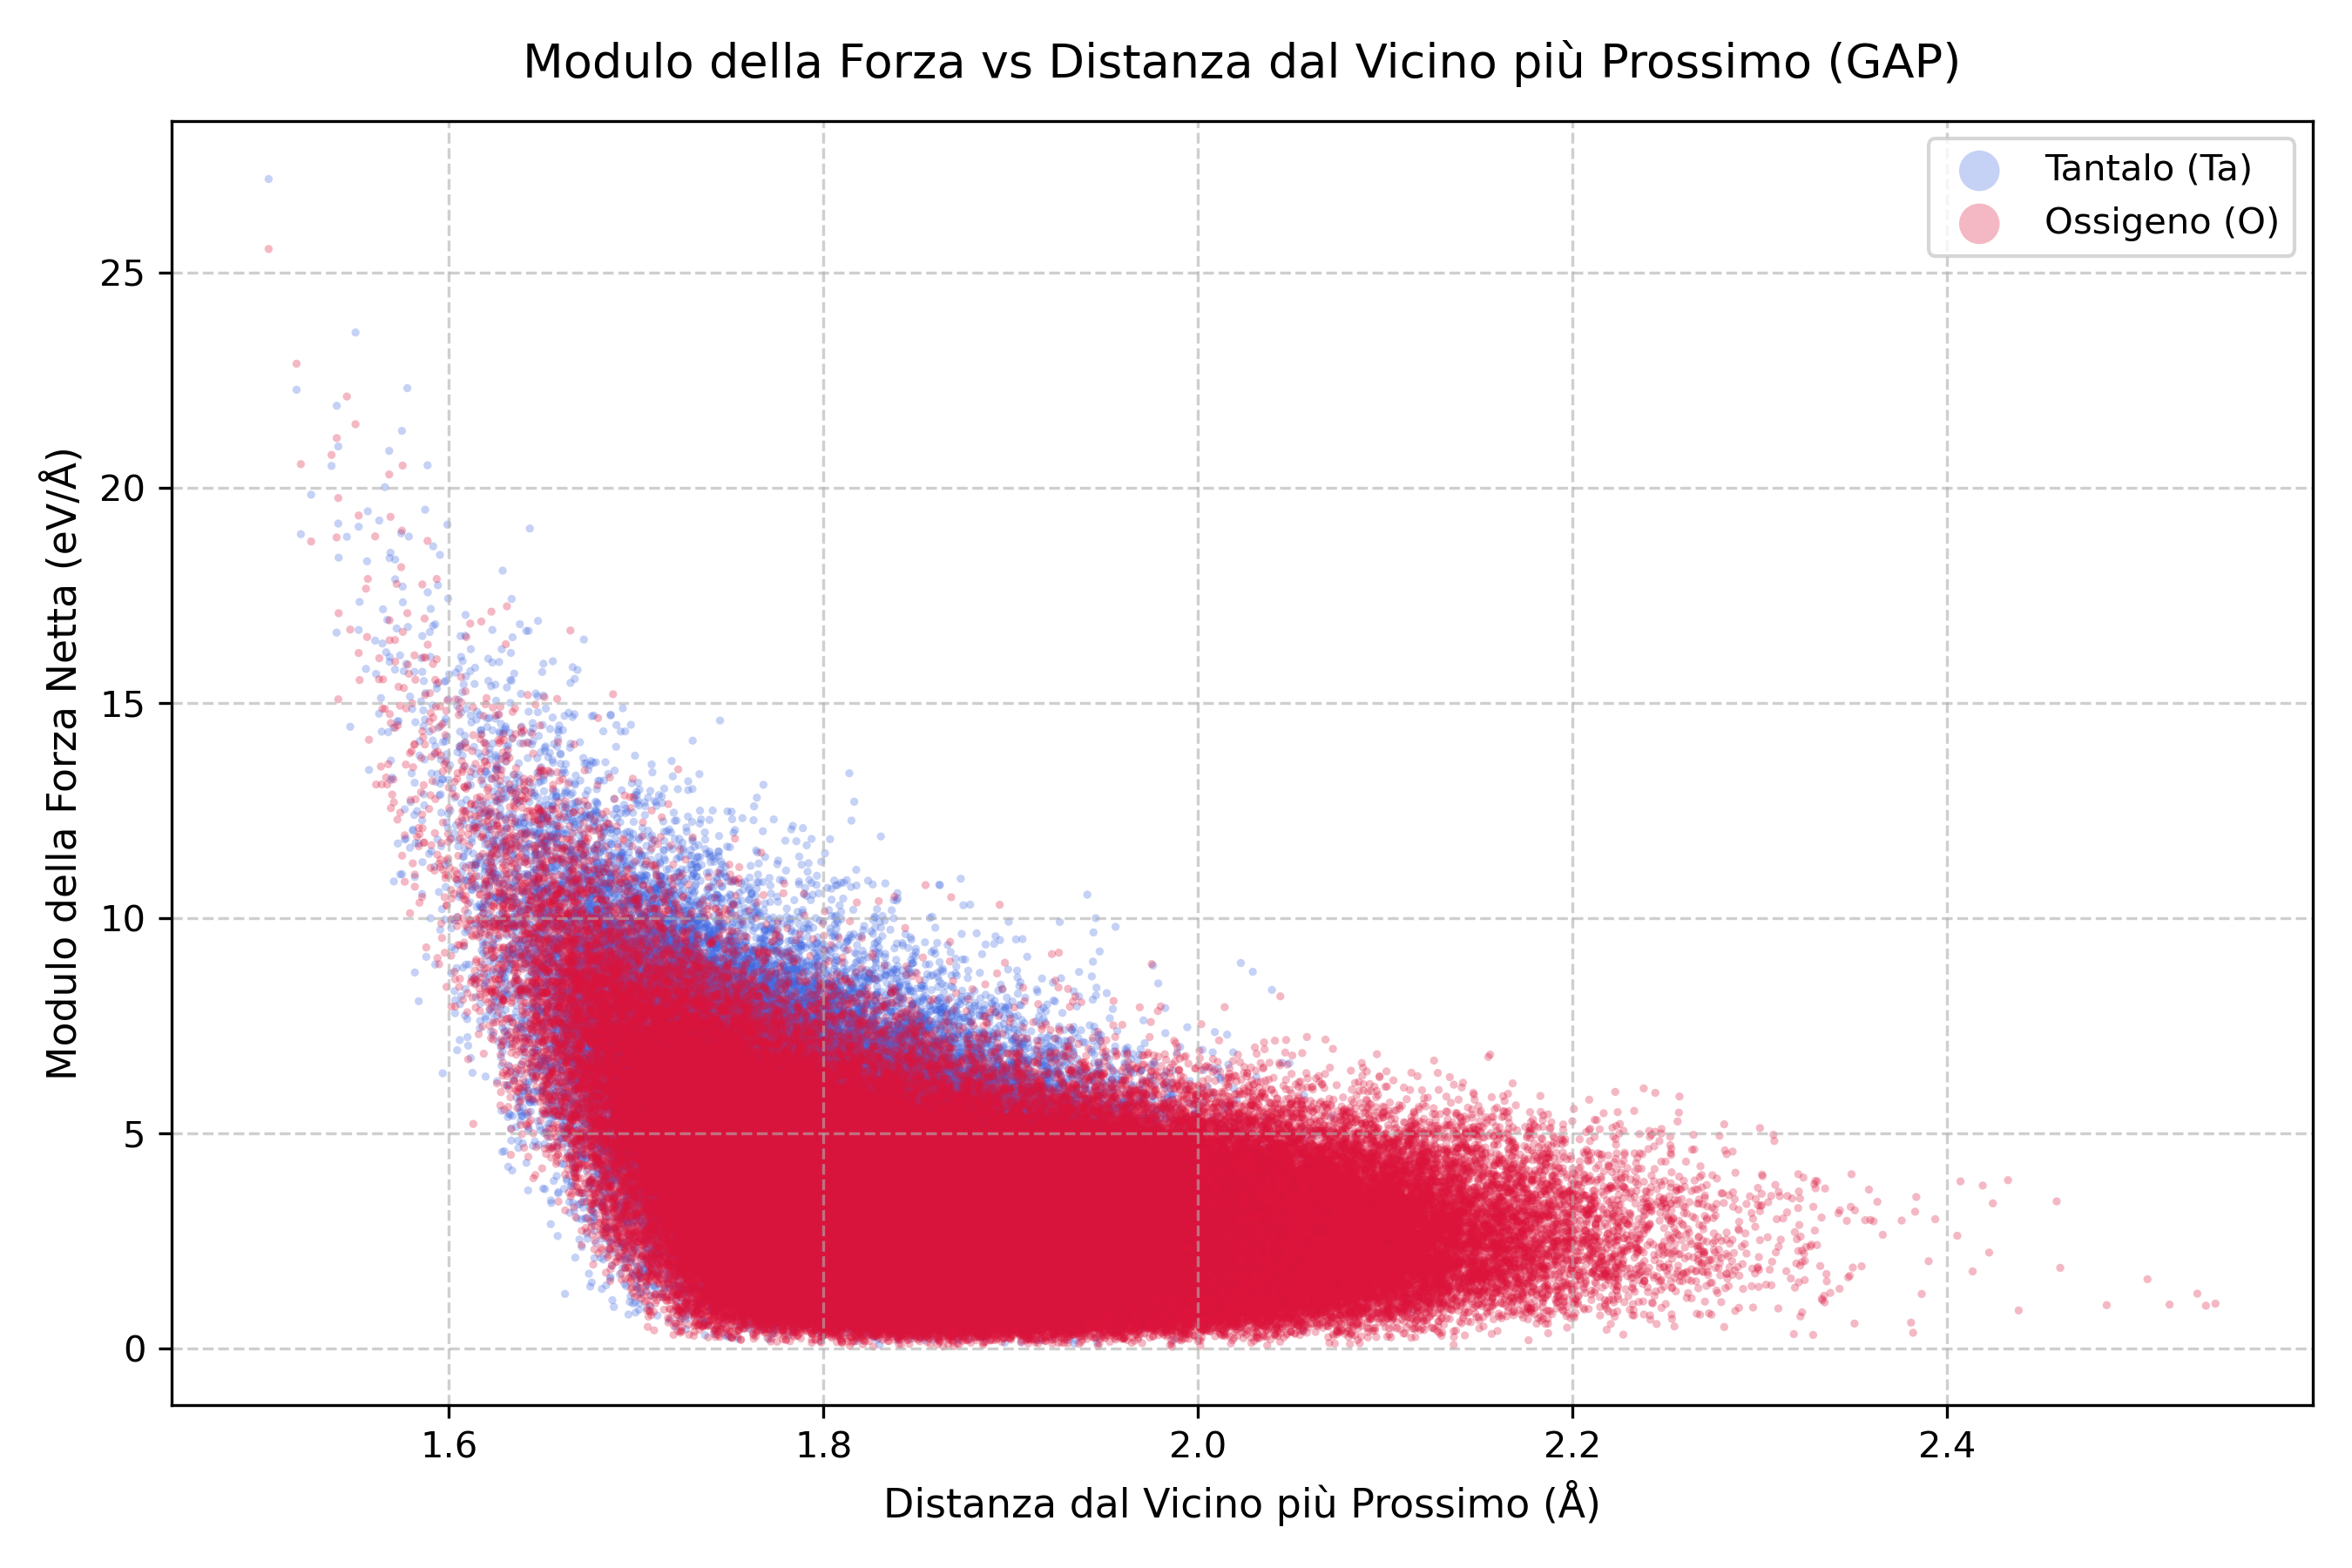
\includegraphics[width=\linewidth]{./img/andamento_forze_totali_distanza_qe_traindata.png}
        \caption{Relazione tra i valori di forza e distanza tra i primi vicini per il set di dati di training}
    \end{subfigure}

    \caption{Distanze e relazione forze distanze per il set di dati di training prodotto con quantum espresso.}
    \label{fig:confronto_forze_distanze_qe_traindata}
\end{figure}
}

quello che notiamo immediatamente, dopo la limitatezza dei valori delle forze, è come la distanza tra i primi vicini assume valori tutti superiori agli $1.5$\AA, inoltre vediamo, che come ci si aspetterebbe, i valori delle forze aumentano alla diminuzione della distanza.


\section{Simulazione con ZBL}

I risultati della sezione precedente sono il principale motivo per il quale andiamo ad addizionare un potenziale repulsivo come lo ZBL.

Anche in questo caso sono stati svolti diversi test, cambiando di volta in volta diversi parametri, non riteniamo necessario riportare tutti questi risultati, inseriamo solo uno di questi, dove l'unica modifica rispetto ai casi precedeti è un timestep di $1$fs.

I parametri per i raggi che abbiamo utilizzato sono dati dal seguente ragionamento, per il $r_{outer} = 1.5$\AA abbiamo deciso di impostare un valore prossimo ai minimi ragistrati nelle configurazioni di training, in questo modo volevamo evitare che lo ZBL si sovrapponesse alle previsioni del GAP. Per quanto riguarda il valore di $r_{inner} = 0.5$\AA abbiamo inserito un valore al quale gli atomi sarebbero sovrapposti e quindi, anche se potrebbe essere alzato, un limite inferiore che dovrebbe essere invalicabile, come si vedrà questo non avviene.

Riportiamo per prima cosa i valori di energia e temperatura

\begin{figure}[h!]
    \centering
    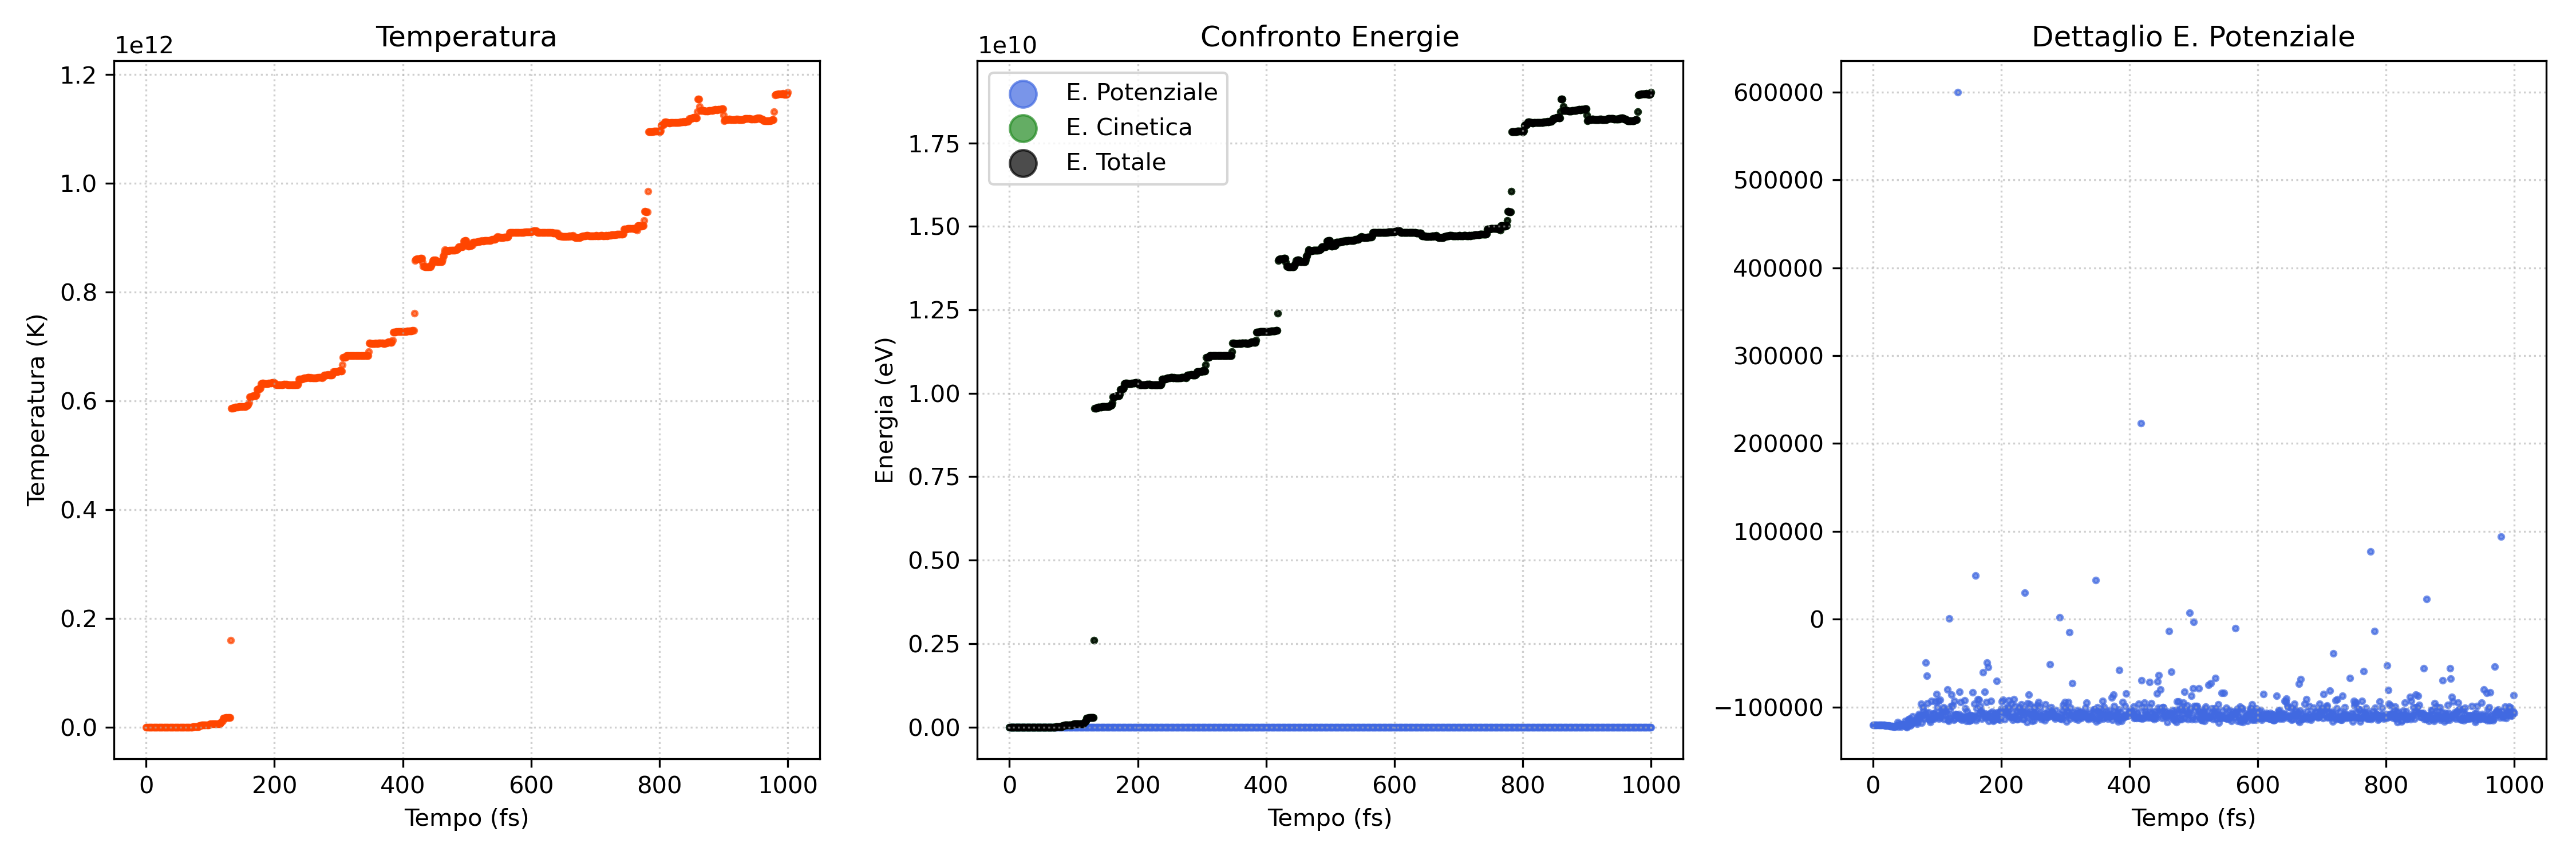
\includegraphics[scale=0.4]{./img/andamento_energia_zbl.png}
    \caption{Grafico dell'andamento temporale per i valori di energia e temperatura, potenziale GAP + ZBL}
    \label{fig:andamento_energia_zbl}
\end{figure}

possiamo vedere come anche in questo caso gli andamenti visti in precedenza si mantengono.

Guardiamo adesso direttamente la relazione tra forze e distanze:

{
\begin{figure}[ht]
    \centering

    \begin{subfigure}{0.48\textwidth}
        \centering
        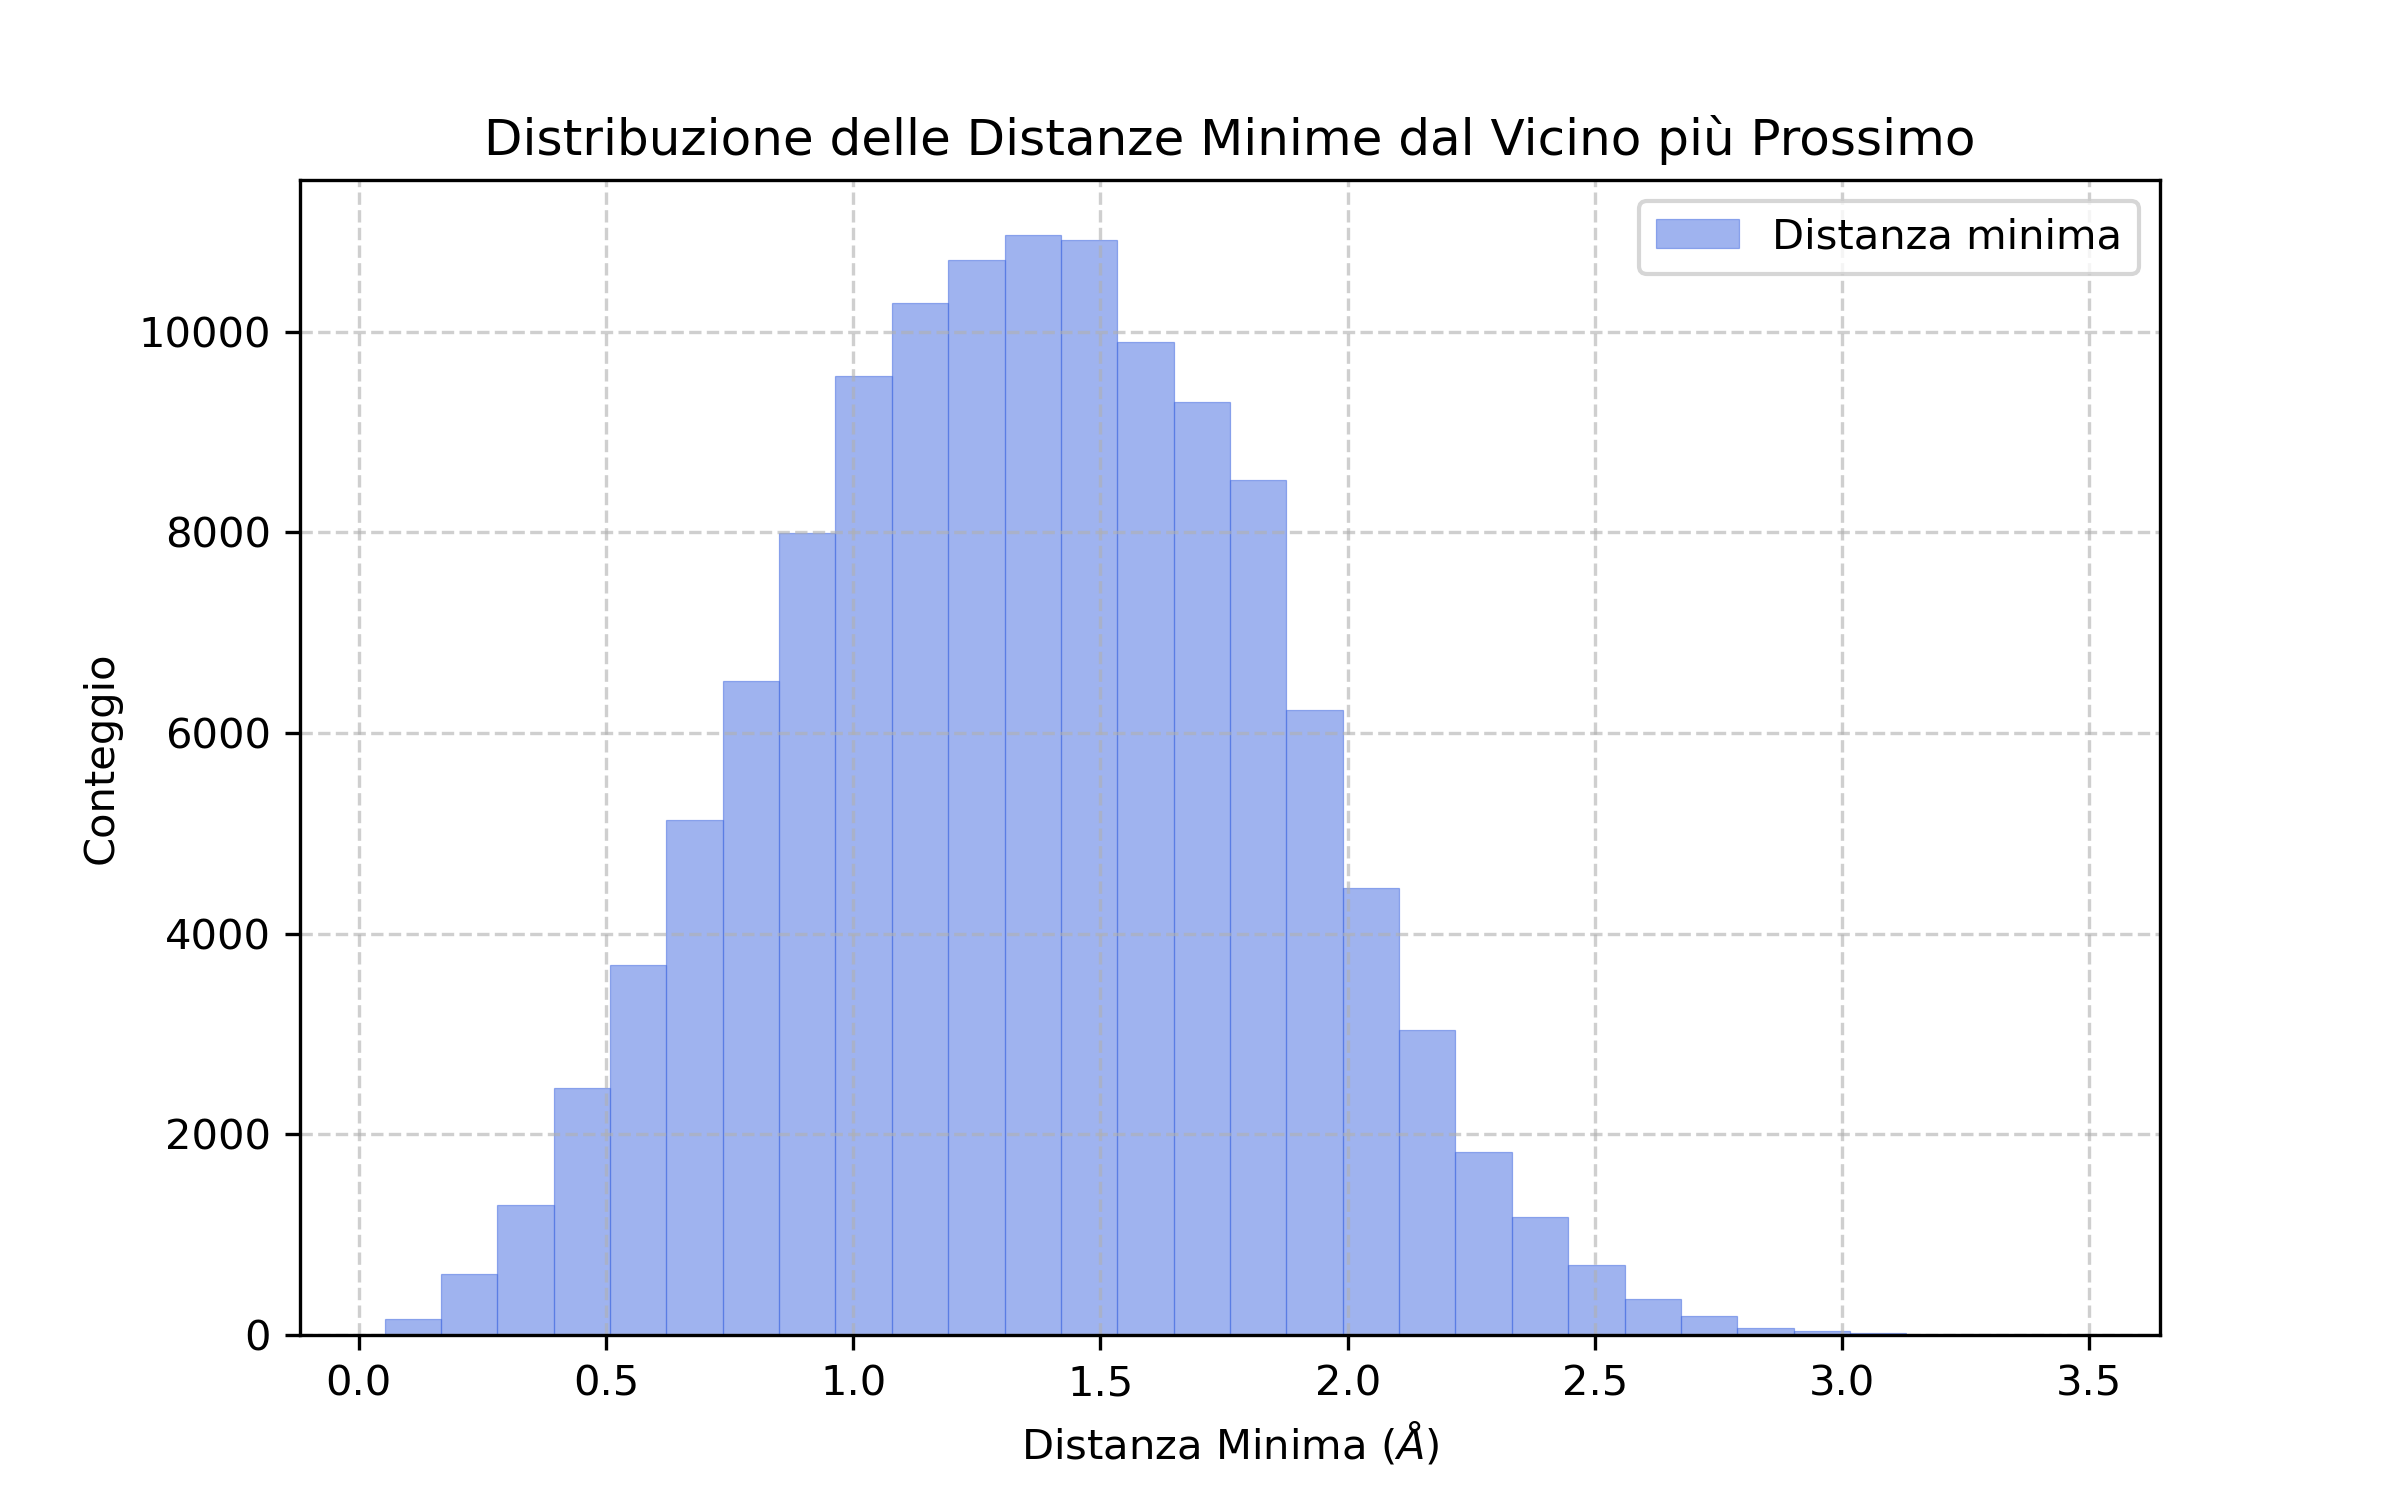
\includegraphics[width=\linewidth]{./img/histo_distanze_zbl.png}
        \caption{Istogramma dei valori di distanza tra i primi vicini per il potenziale GAP + ZBL}
    \end{subfigure}
    \hfill
    \begin{subfigure}{0.48\textwidth}
        \centering
        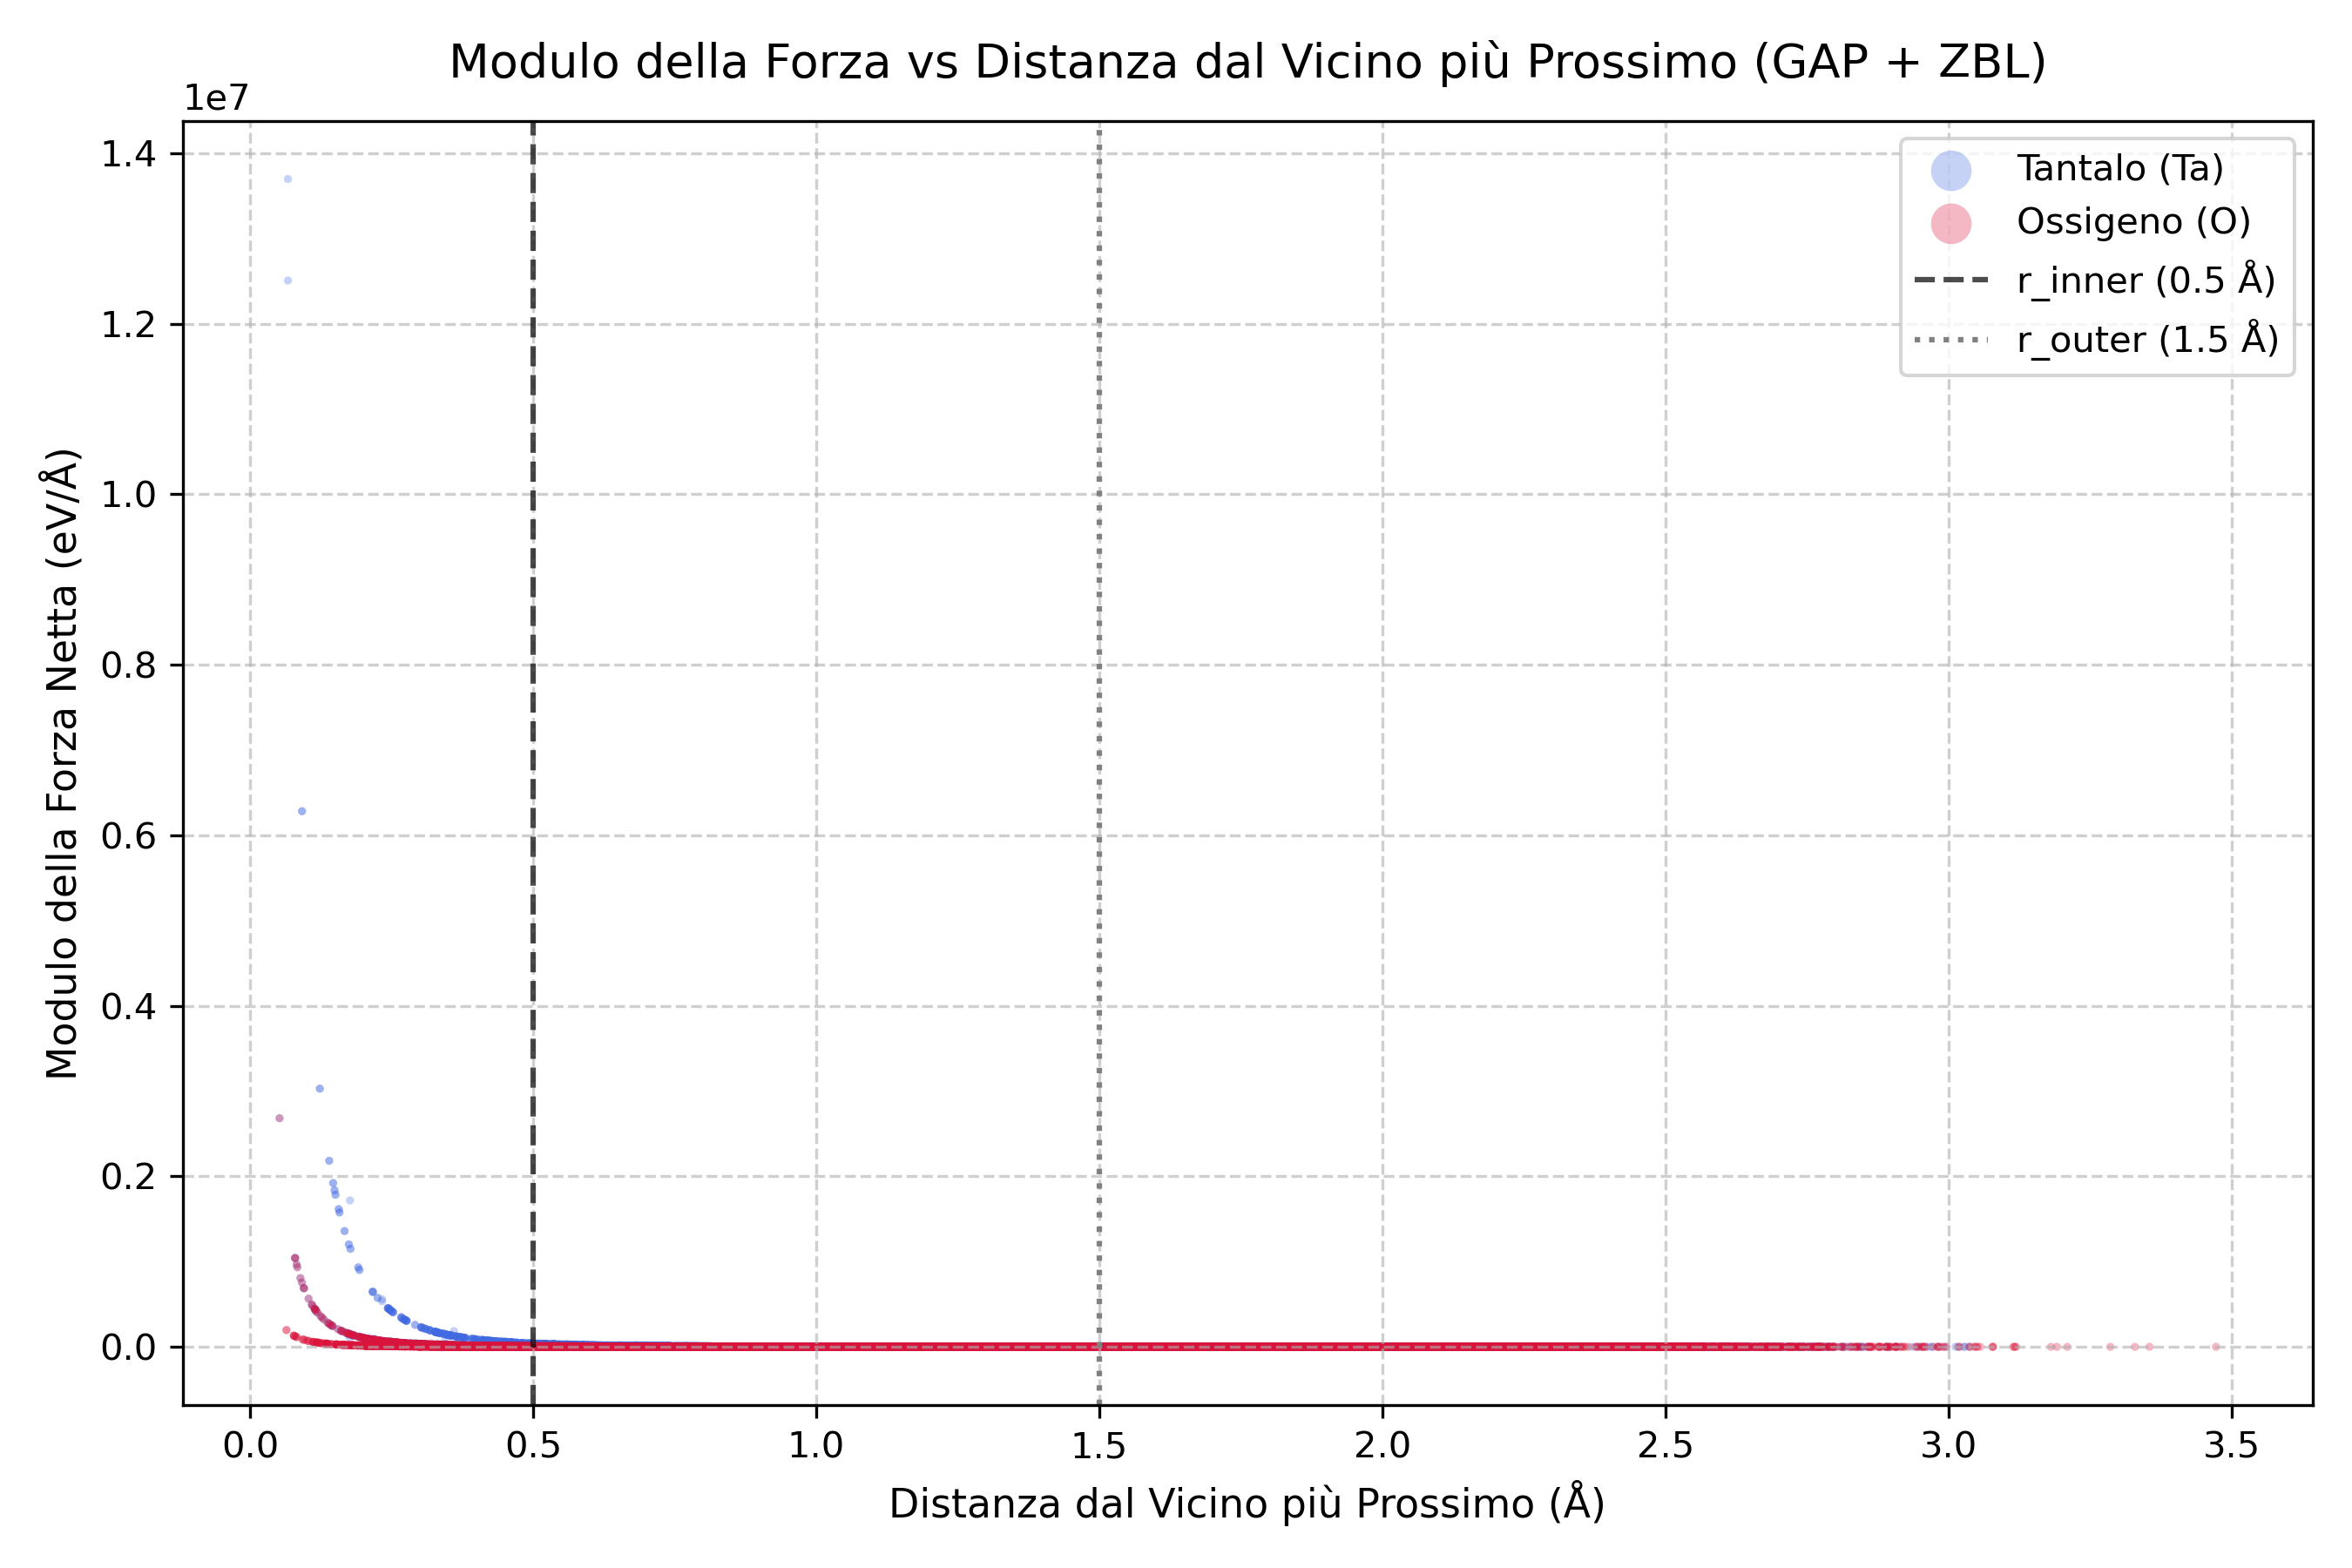
\includegraphics[width=\linewidth]{./img/andamento_forze_totali_distanza_zbl.png}
        \caption{Relazione tra i valori di forza e distanza tra i primi vicini per il potenziale GAP + ZBL}
    \end{subfigure}

    \caption{Distanze e relazione forze distanze per il potenziale GAP + ZBL.}
    \label{fig:confronto_forze_distanze_qe_traindata}
\end{figure}
}

in questo caso è anche utile guardare al confronto tra i due contributi di forza

\begin{figure}[h]
    \centering
    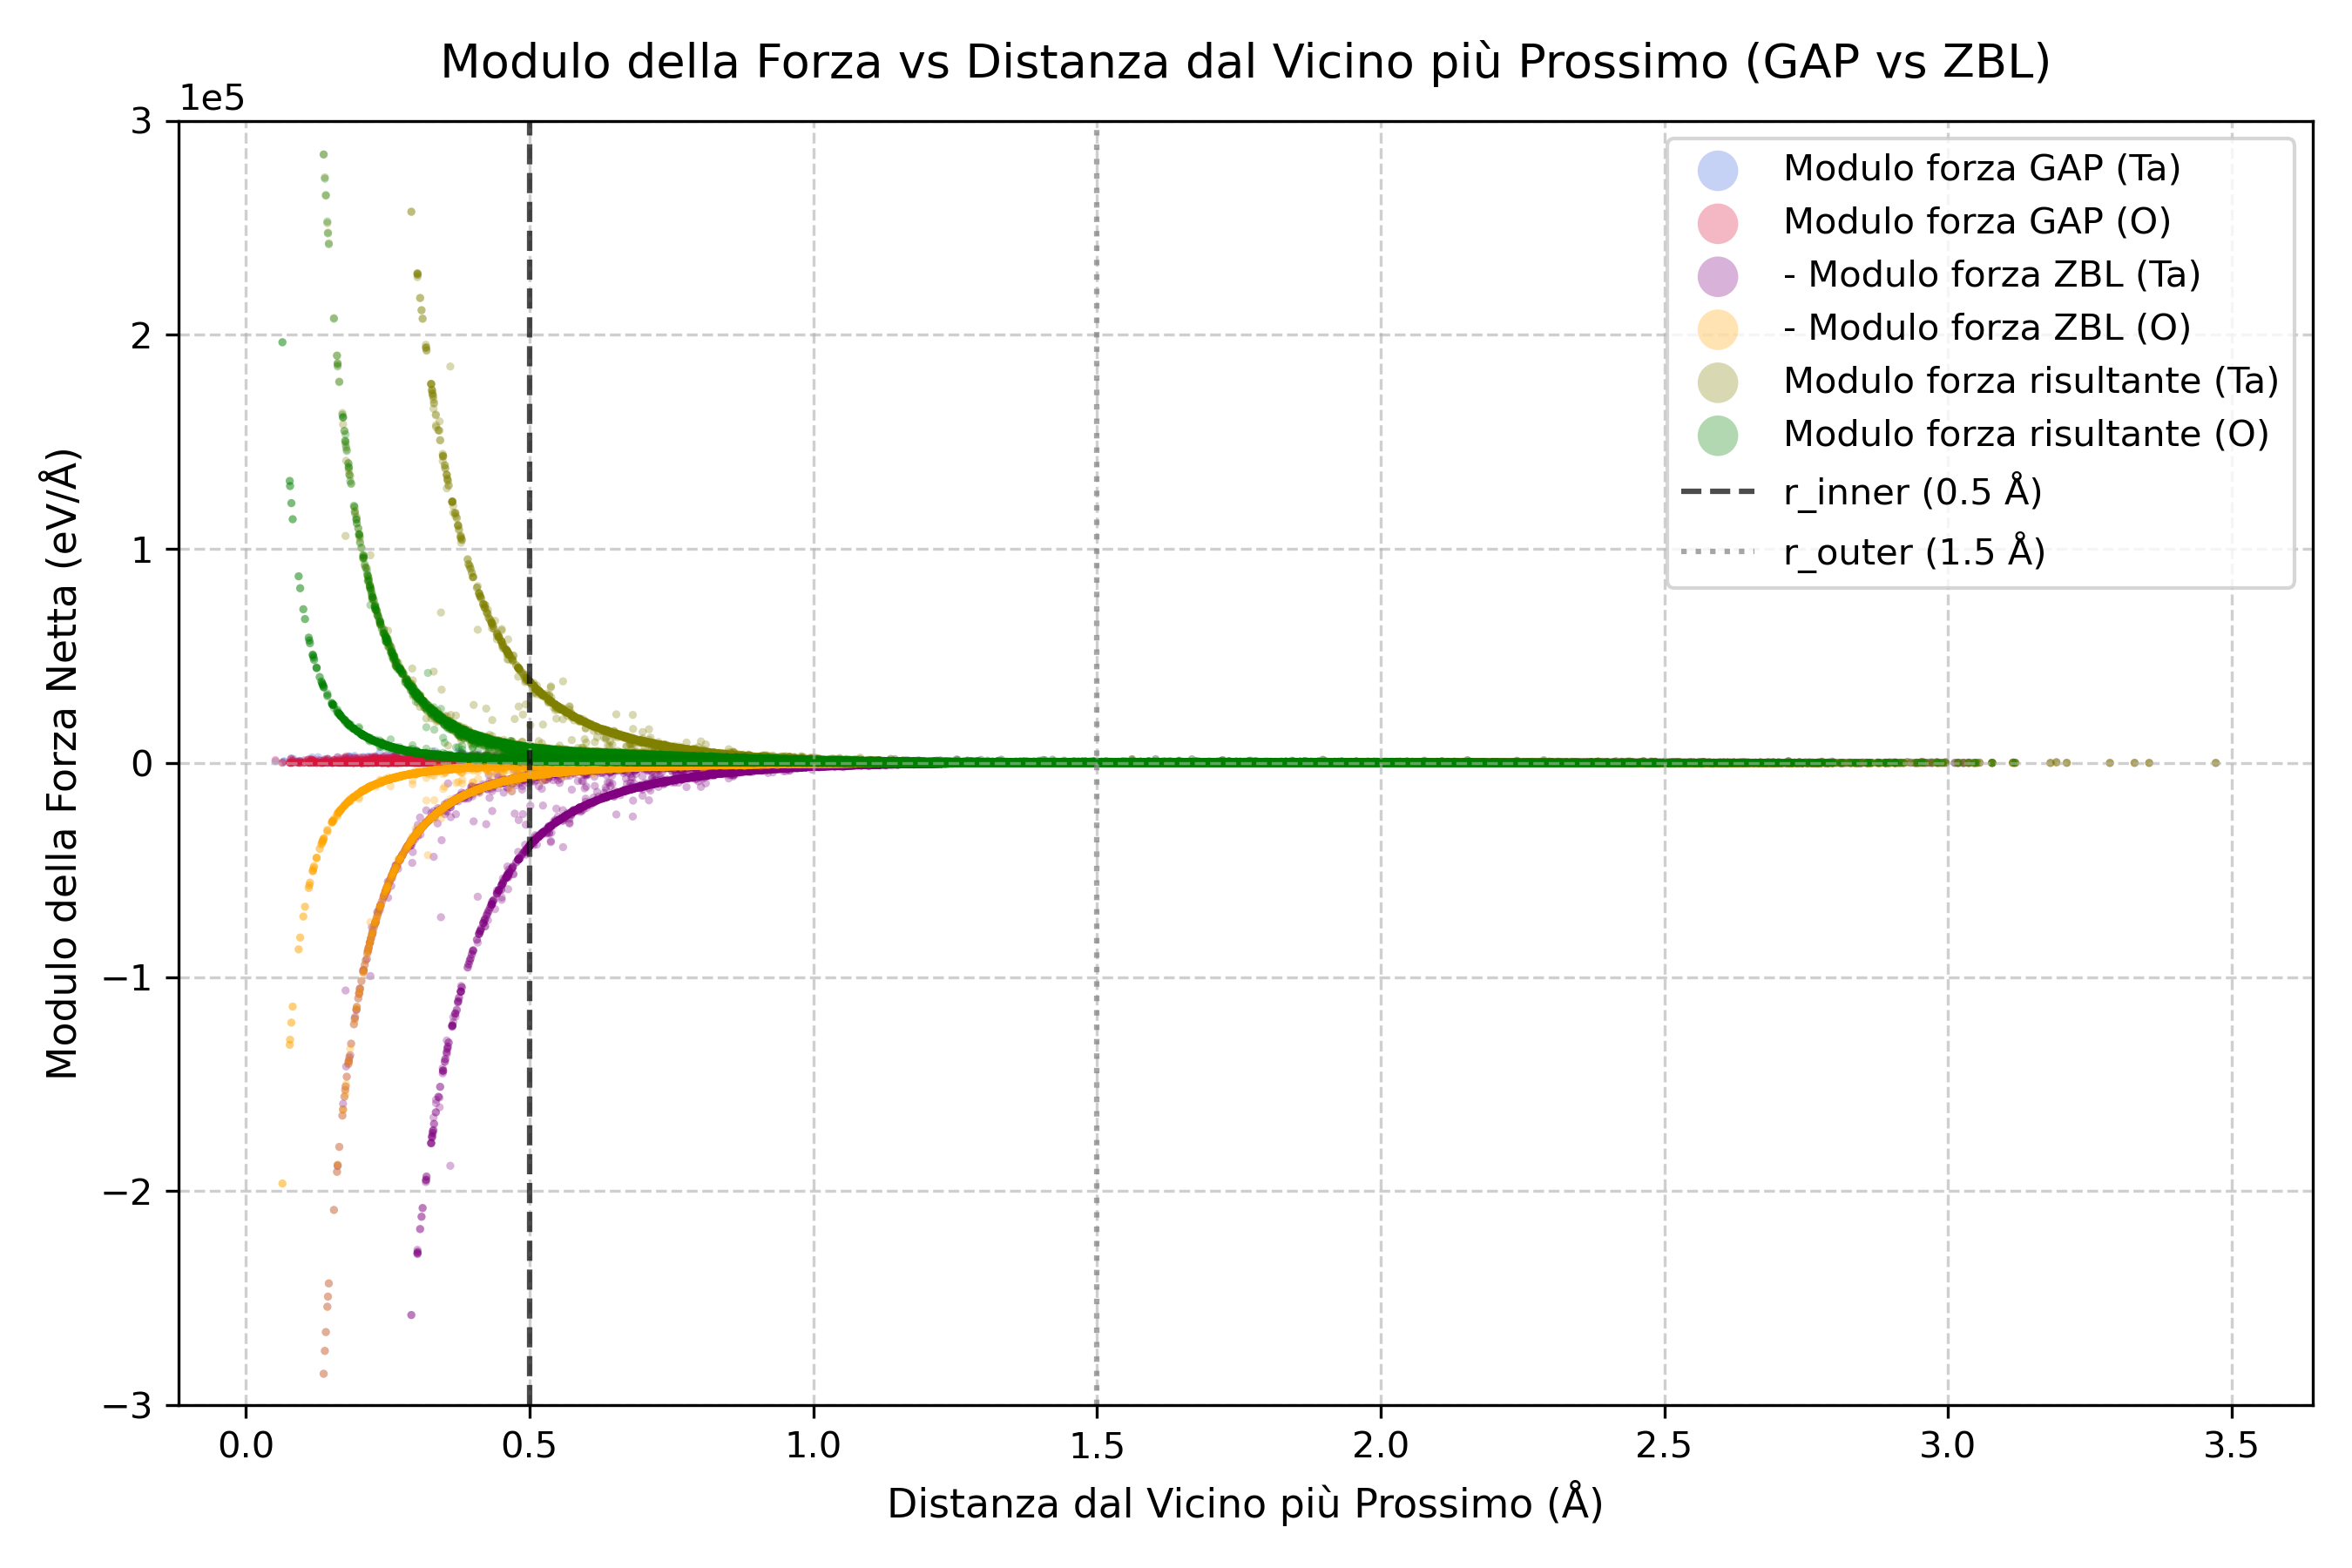
\includegraphics[scale=0.4]{./img/confronto_forze_vs_distanza_minima_zbl.png}
    \caption{Grafico del confronto tra i contributi di forza di GAP e di ZBL}
    \label{fig:confronto_forze_vs_distanza_minima_zbl}
\end{figure}

possiamo notare come i valori di distanza tra i primi vicini arrivino comunque sotto la soglia imposta come minima. Proporniamo come spiegazione di questo fenomeno il fatto che la correzione dello ZBL non sia adeguata a compensare i valori prodotti dal potenziale GAP, essendo questi molto distanti dalle configurazioni di training. Inoltre vogliamo far notare come i moduli delle forze a distanze piccoli siano dati quasi totalmente dalla repulsione prodotta dallo ZBL, questo ci permette di confermare il suo comportamento adeguato, in conclusione non è immediatamente chiaro il motivo per il quale questa correzione non porti a risulati più in linea con le previsioni fatte.

\section{Simulazione con metodo Montecarlo}



